\documentclass[11pt]{article}		% Sets font size and document type
\usepackage{fontspec}				% Allows us to use custom fonts
\usepackage{graphicx}				% Does pictures
\usepackage{parskip}				% Removes paragraph indents
\usepackage{multicol}				% Allows for multiple columns
\usepackage{titlesec}				% Changes section title appearance
\usepackage{setspace}				% Allows you to set line spacing
\usepackage{amsmath}				% Maths typesetting
\usepackage[margin=20 mm]{geometry}	% Sets page margin
\usepackage[colorlinks=true,linkcolor=blue,citecolor=blue,urlcolor=blue]{hyperref}	
									% Allows for hypertext for references (links) - edited to hake links look like normal text rather than having a border
\doublespacing						% Double spaces - this annoys me but is unavoidable I think

% Makes it so all equations have full sized numbers, independent of font size used		
\makeatletter
\def\tagform@#1{\maketag@@@{\normalsize(#1)\@@italiccorr}}
\makeatother


%Add any more packages needed here:
\usepackage[justification=centering,font=small]{caption}	
									% Centres captions and makes them smaller
\usepackage[none]{hyphenat}			% Lines end cleanly - no hyphenation mid word
\usepackage{fancyhdr}				% Nicer headers/footers
\usepackage{amssymb}				% Allows for more maths symbols including not less than

% There is some scope for changing the paragraph spacing and spacing around section headers if you are short of space

\graphicspath{{Images/}}	% Images are in a folder called 'Images'

% Set a variable for image height, so all images are the same size and easy to change
\newlength{\imageheight}	 % Creates the variable
\setlength{\imageheight}{0.35\textwidth}  % Sets the variable

% Use Arial
\setmainfont[
BoldFont=Arial Bold.ttf,
ItalicFont=Arial Italic.ttf,
BoldItalicFont=Arial Bold Italic.ttf
]{Arial.ttf}

% Have got this working with TexStudio now - need to change compiler from default to XeLaTeX (Options > Configure TexStudio > Build > Default Compiler > XeLaTeX)
% Will be slow at first, but once the fonts have installed should work more quickly

% Overleaf link - https://www.overleaf.com/project/5fce665153f1701e8414d47b

\begin{document}
	
	\flushleft
	\raggedright

	\begin{center}
		\vspace*{2cm}
		Michaelmas \& Hilary Term 2020 / 2021\\ % enter the date
		\vspace*{6cm}
		\huge{\textbf{3YP Project: Pipe Inspection Robot}}\\ 
		\vspace*{6cm}
		\large{Monty Beresford, Louis Emanuel, Joshua Gei \& Jim Laney} % Not your Bod card number
		\thispagestyle{empty} % Remove page number
	\end{center}

	\newpage
	
	\tableofcontents
	\thispagestyle{empty} % Remove page number
	\newpage

	\setcounter{page}{1}
	
	\section{Introduction}
	
	\subsection[Product Description]{Product Description - Jim Laney}
	The pipe inspection robot works in underground pipes in urban areas, with a pipe diameter from $609.6$ mm to $914.4$ mm and with pipes at any angle, providing a map of the pipe with the location of any failures to the operator. % 24 - 36 inches; Needs citation for pipe sizes?
	The robot reduces the disruption caused by having to dig up large areas of pipe for inspection, since the issue can be located and smaller, less disruptive work can be undertaken.
	It is intended to provide an inspection method for pipes which cannot be inspected by the current leading method, Pipe Inspection Gauges (PIGs), which only work in horizontal or near horizontal straight pipes\textsuperscript{\cite{mills2017advances}}.
	It enters a pipe using a launch tube, and travels autonomously along the inside of the pipe, checking for evidence of cracks and corrosion and logging their location for future maintenance.
	\\
	
	\begin{figure}[h] % Would like to do this as a text wrapped figure but that can be finnicky so would like to agree on this as a group before attempting it
		\centering
		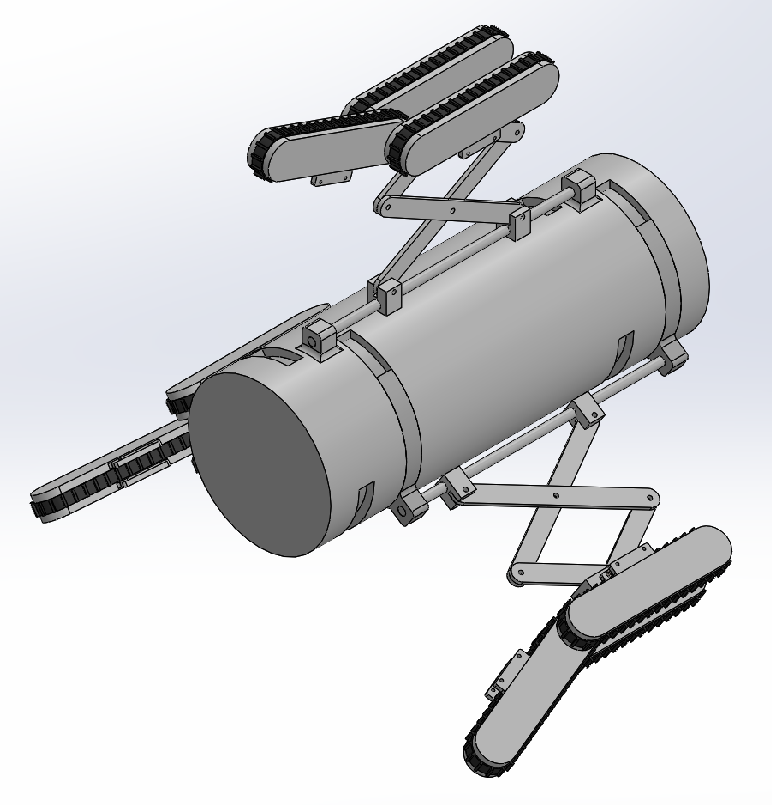
\includegraphics[height=\imageheight]{overviewCAD}
		\caption{3D CAD model of robot}
		\label{3DSketch}
	\end{figure}
	
	While inside the pipe, the robot uses three legs to maintain contact and provide the required normal force to move inside the pipe, as shown in \hyperref[3DSketch]{Figure \ref*{3DSketch}}.
	Two of these legs can be rotated to provide improved speeds over pipes at different angles, and all three legs can be extended and retracted to fit the pipe diameter the robot is currently in.
	It can navigate around bends and through pipes at different angles, without prior knowledge of the location or angle of these, and will automatically feedback to the control system in order to create an accurate map.
	\\
	The robot uses computer vision to identify cracks and corrosion, allowing it to mark where these occur for human maintenance, and then combines this with knowledge of its position to create a map of the pipe it has travelled and where issues have occurred.
	It can transmit its location using a small transmitter, which has a separate power supply so that if the robot breaks down it can be located with minimal excavation.
	
	\subsection[Patent Analysis]{Patent Analysis - Jim Laney}
	
	It was decided to look at patents classified as \verb|F16L55/26| - "Pigs or moles, i.e. devices movable in a pipe or conduit with or without self-contained propulsion means" or \verb|F16L2101/30| - "Inspecting, measuring or testing [as a use or application of pigs or moles]" as these are most similar to the purpose which our robot fulfils.
	In these patents the use of "pigs" refers to Pipeline Inspection Gauges (PIGs from here on), and moles are used as a synonymous term, and will thus also be referred to as PIGs from now on.
	While our robot is not a PIG as PIGs are typically unpowered and cannot deal with bends in the pipe, this is the closest patent classification which we can consider.
	\begin{figure}[h]
			\centering
			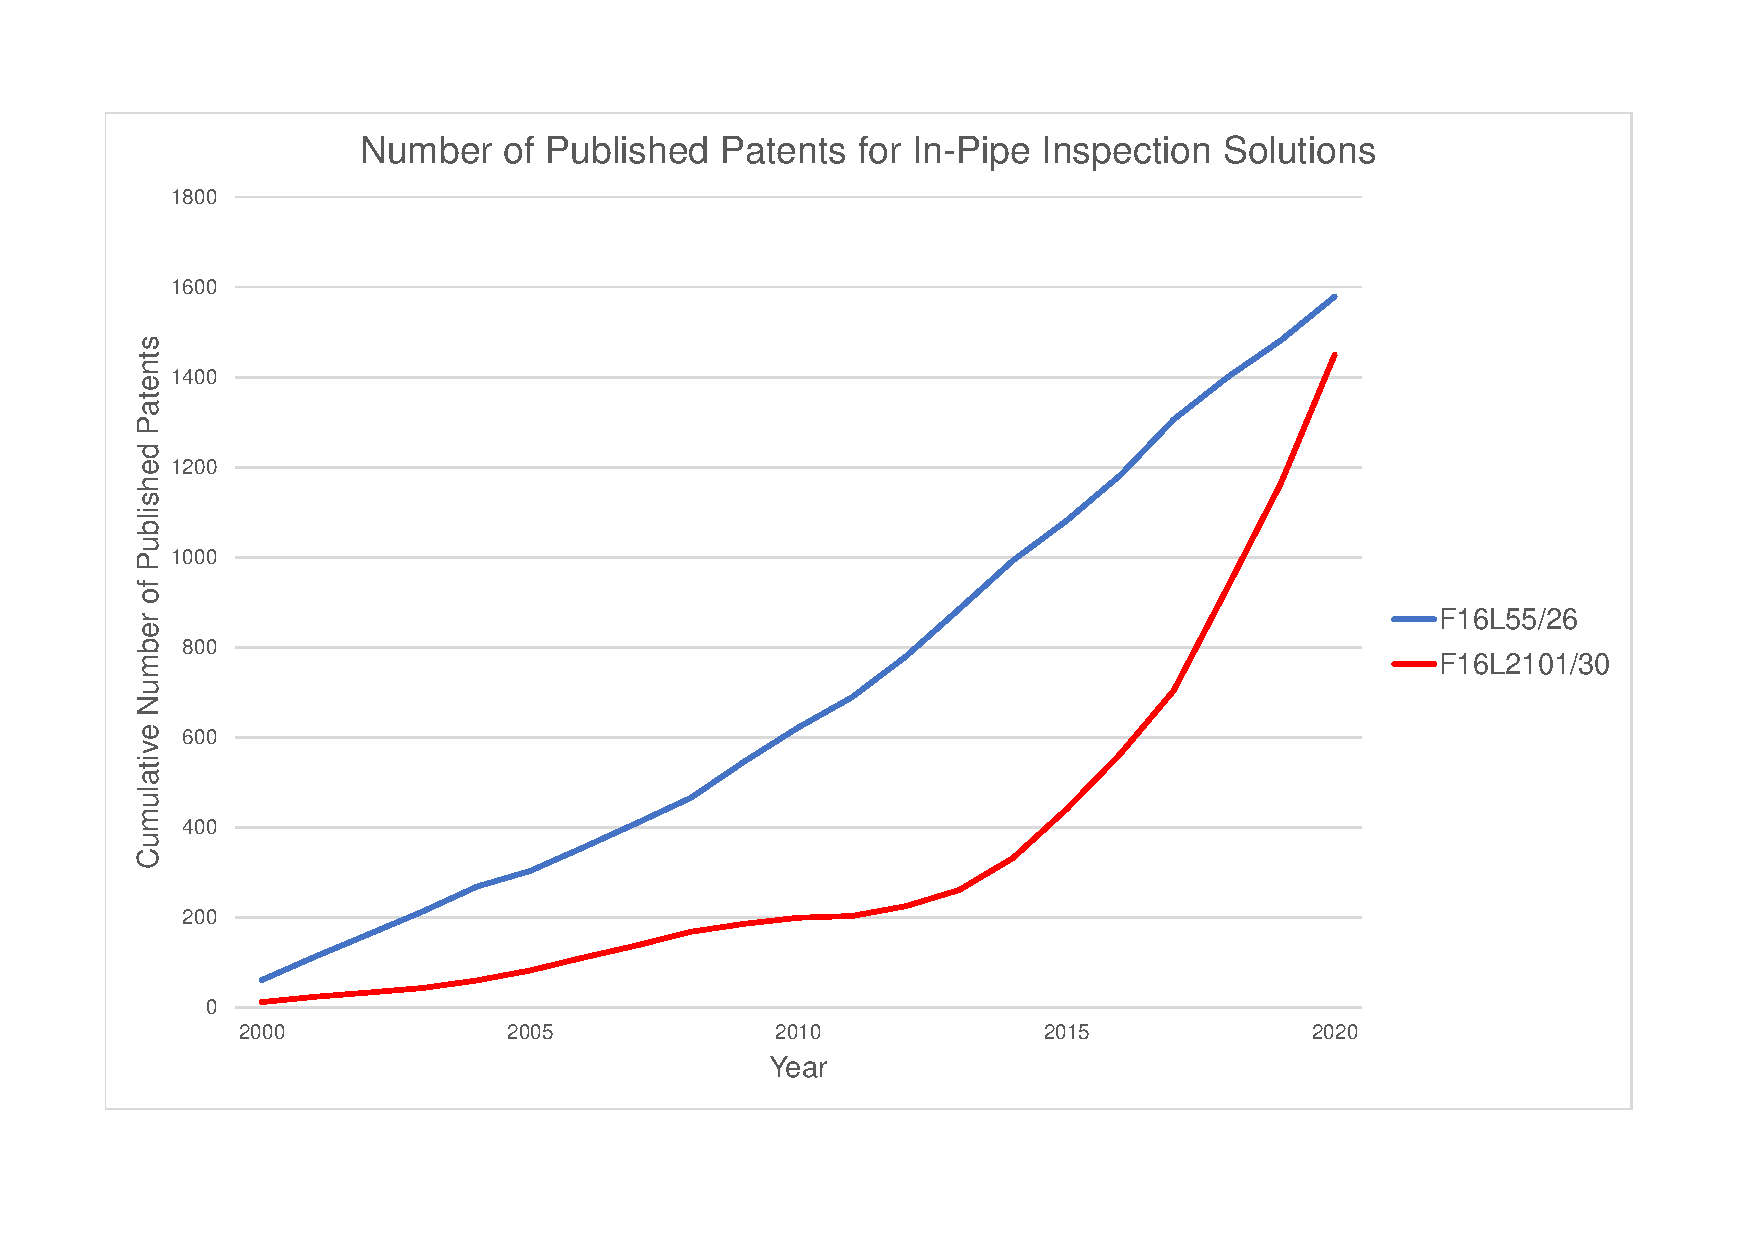
\includegraphics[height=\imageheight]{patentGraph}
			\caption{Cumulative number of published patents in the European Patent Office database classified as \texttt{F16L55/26}\textsuperscript{\cite{patent26}} or \texttt{F16L2101/30}\textsuperscript{\cite{patent30}} }
			\label{patentGraph}
	\end{figure}
	\\
	As you can see from \hyperref[patentGraph]{Figure \ref*{patentGraph}}, the rate of patent publication in both classifications is still growing at a rapid rate, suggesting the technology is in a period of rapid innovation and development.
	This suggests that industry is still in the initial period of product design ferment, where no dominant design has occurred\textsuperscript{\cite{christensen1998innovation}}.
	Thus there is a much greater chance of survival, as this dominant design has not yet been established, and the space for new innovators is greater.
	While there is also a risk to entering the industry too early, we believe that period has passed, due to the sustained period of development in the last 20 years.
	
	
	\section{Hardware}
	
		\subsection[Locomotion]{Locomotion - Jim Laney}
			
			%By Jim
			The main locomotion of the robot is a set of 3 legs with a pantograph mechanism  to allow for the adaptation to different diameters, with tracks at the end to drive the motion, as shown in \hyperref[legDesign]{Figure \ref*{legDesign}}.
			There is one leg which remains stationary at the top of the robot, and two legs which are able to rotate about the body of the robot between $20^\circ$ and $90^\circ$ to the vertical.
			At the end of each leg there is a passive joint between the leg and the track to allow for the robot to travel along surfaces which are not perpendicular to the legs, such as around bends or over uneven surfaces.
			\\
			The length of the pantograph is controlled by the force from two opposing linear actuators, which extend to a given length to set the distance of the pantograph.
			The track at the end of the pantograph is connected to a freely turning joint, which can be measured using two angular encoders to give the angle $\phi$, shown in \hyperref[legDiagram]{Figure \ref*{legDiagram}}, with the springs acting to restore $\phi$ to $0^\circ$ when under no external effects.
			In addition to this, the tracks use an active compliance joint, as shown in \hyperref[activeCompliance]{Figures \ref*{activeCompliance} \& \ref*{unevenBehaviour}}, which allows for the robot to maintain maximum surface contact at all times.
			\\
			The active compliance joint consists of a torsional spring and radio-controlled servo motor, which are both attached around the same axis.
			However, the servo motor is attached to the rear tracks, whereas the spring is attached between the front track and the servo motor itself.
			When the robot passes over an uneven surface, the servo motor forces the front track down, maintaining contact with the pipe wall, as shown in \hyperref[unevenBehaviour]{Figure \ref*{unevenBehaviour}(a)}
			If instead the robot is in a section where the pipe wall is concave, the torsional spring will allow it to fold, shown in \hyperref[unevenBehaviour]{Figure \ref*{unevenBehaviour}(b)}, and maintaining contact with as much of the wall as possible.
			The active compliance joint also includes an angular encoder to tell how much the front track has been bent, allowing for the active compliance joint to be better controlled.
			\begin{figure}[h]
				\centering
				\begin{multicols}{2}
					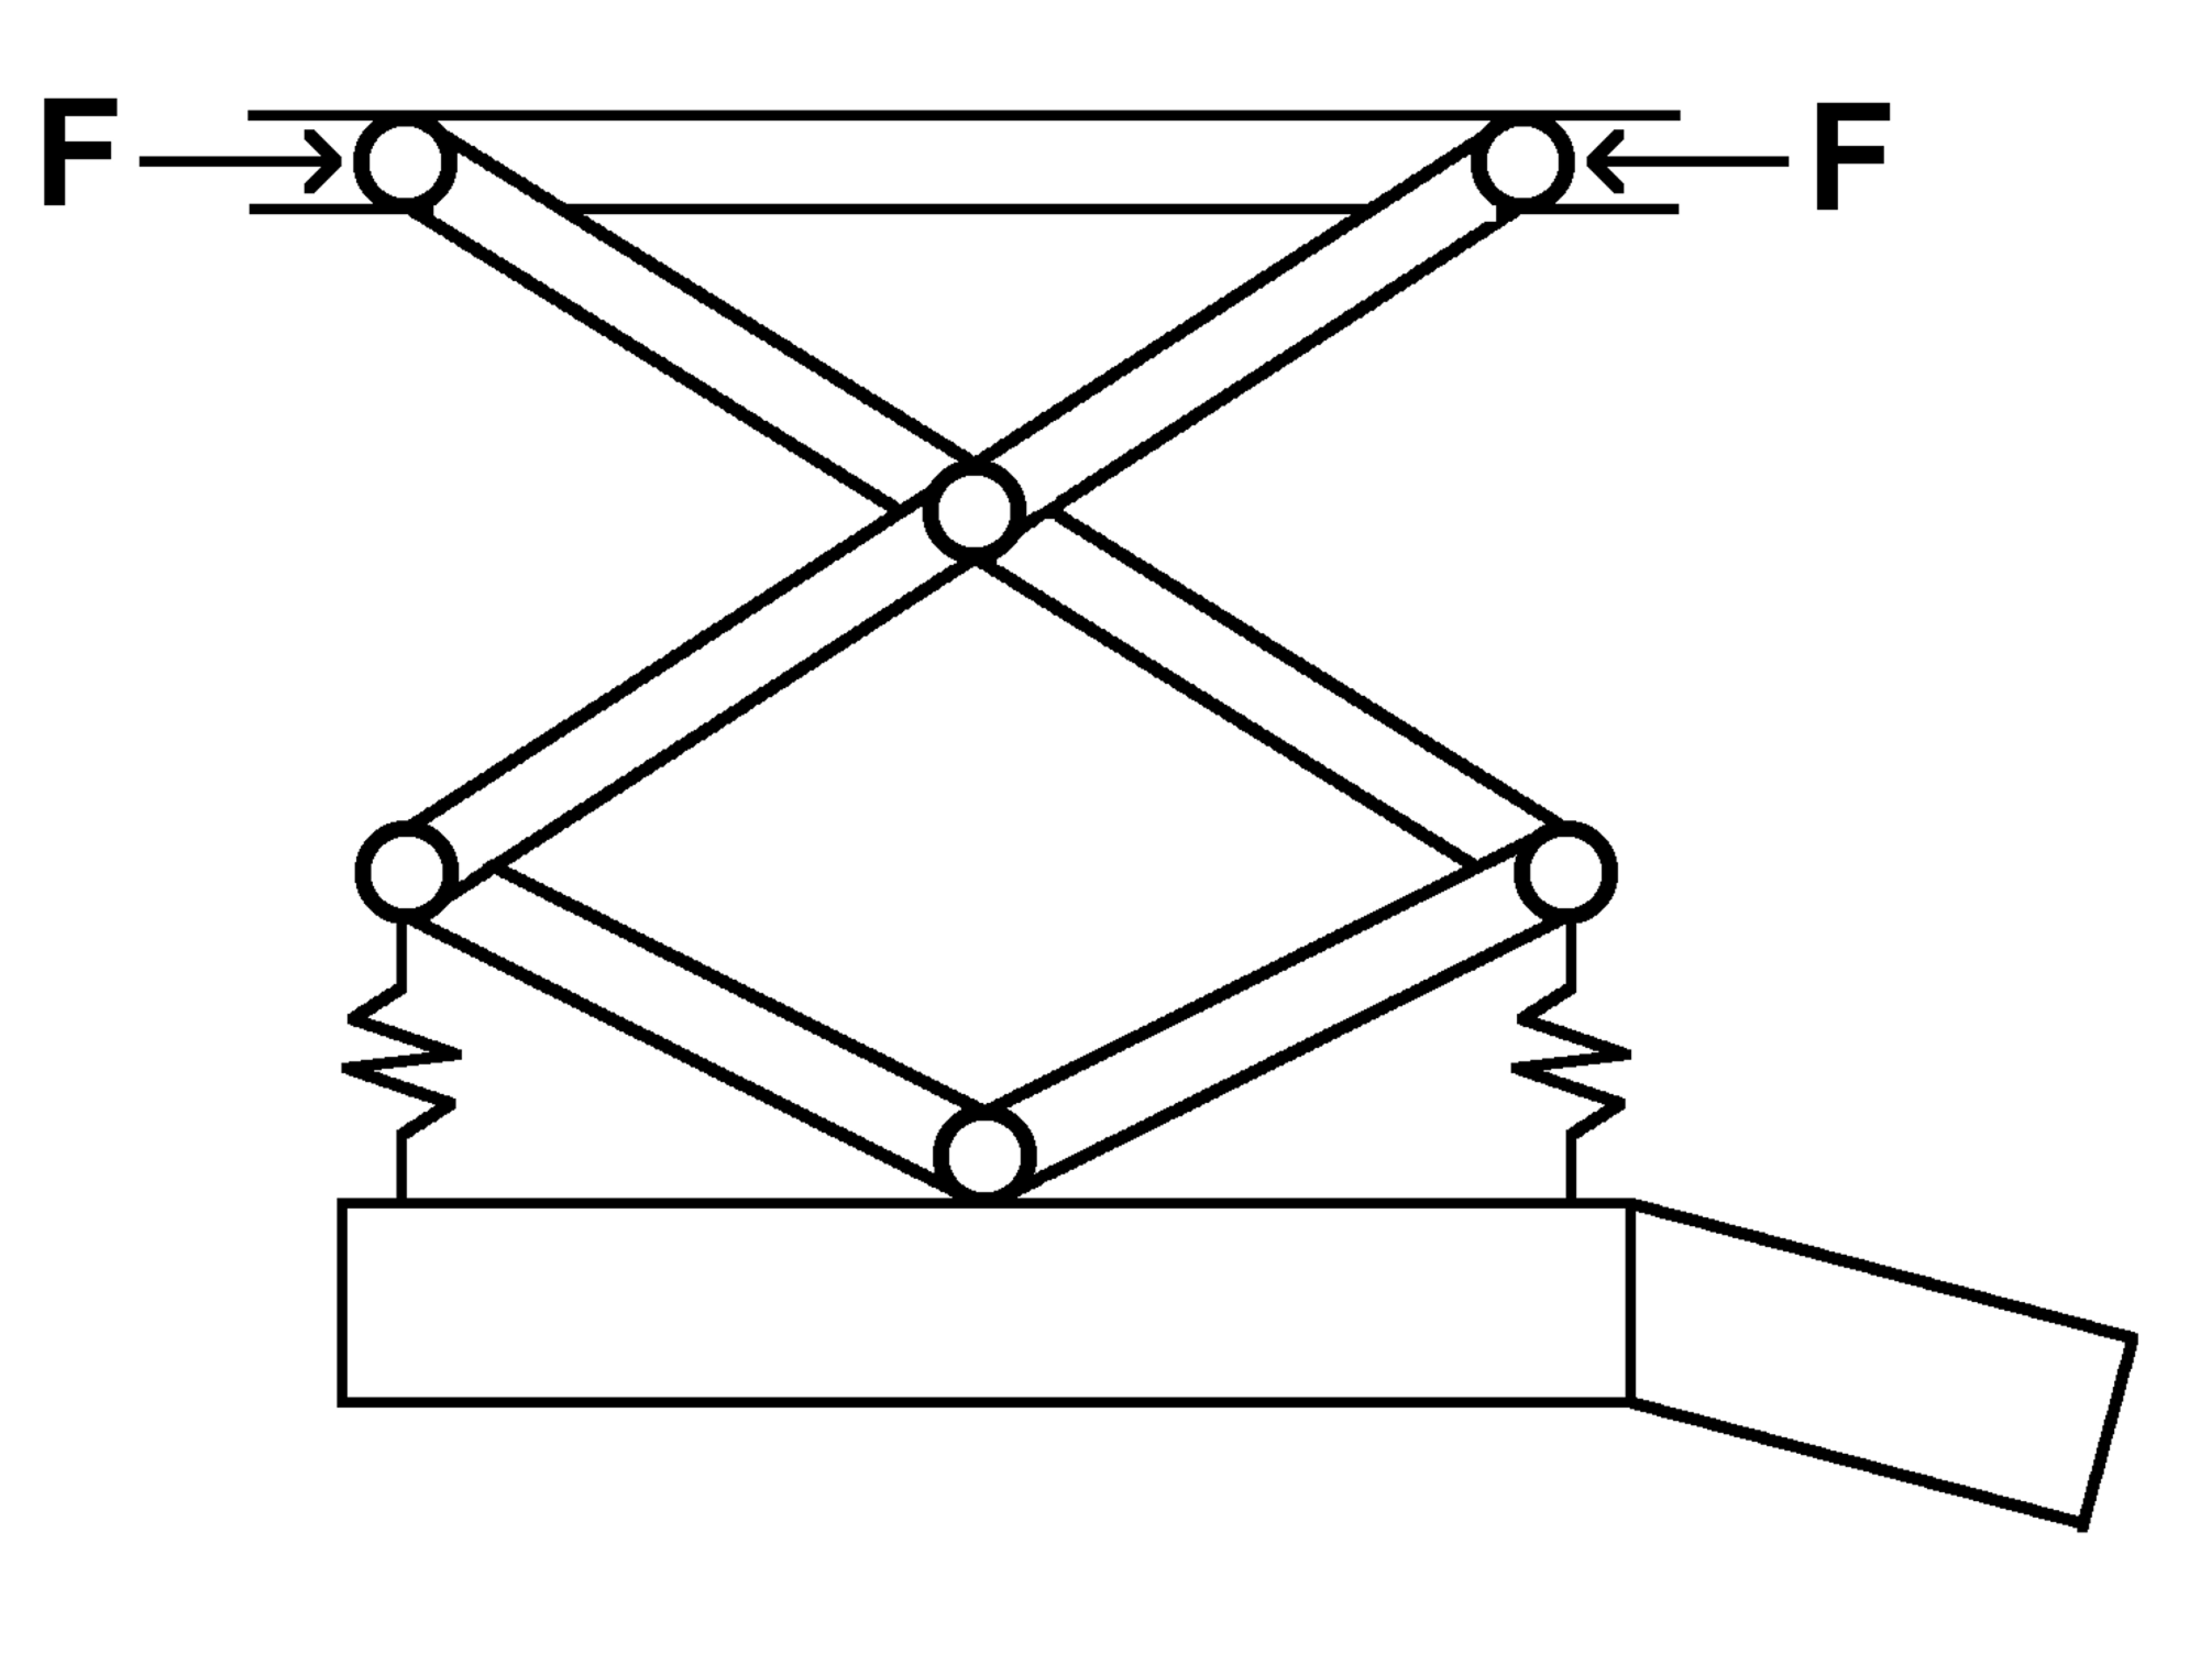
\includegraphics[height=\imageheight]{legDesign}
					\caption{Diagrammatic representation of the pantograph mechanism used for the robot's legs}
					\label{legDesign}
					\columnbreak
					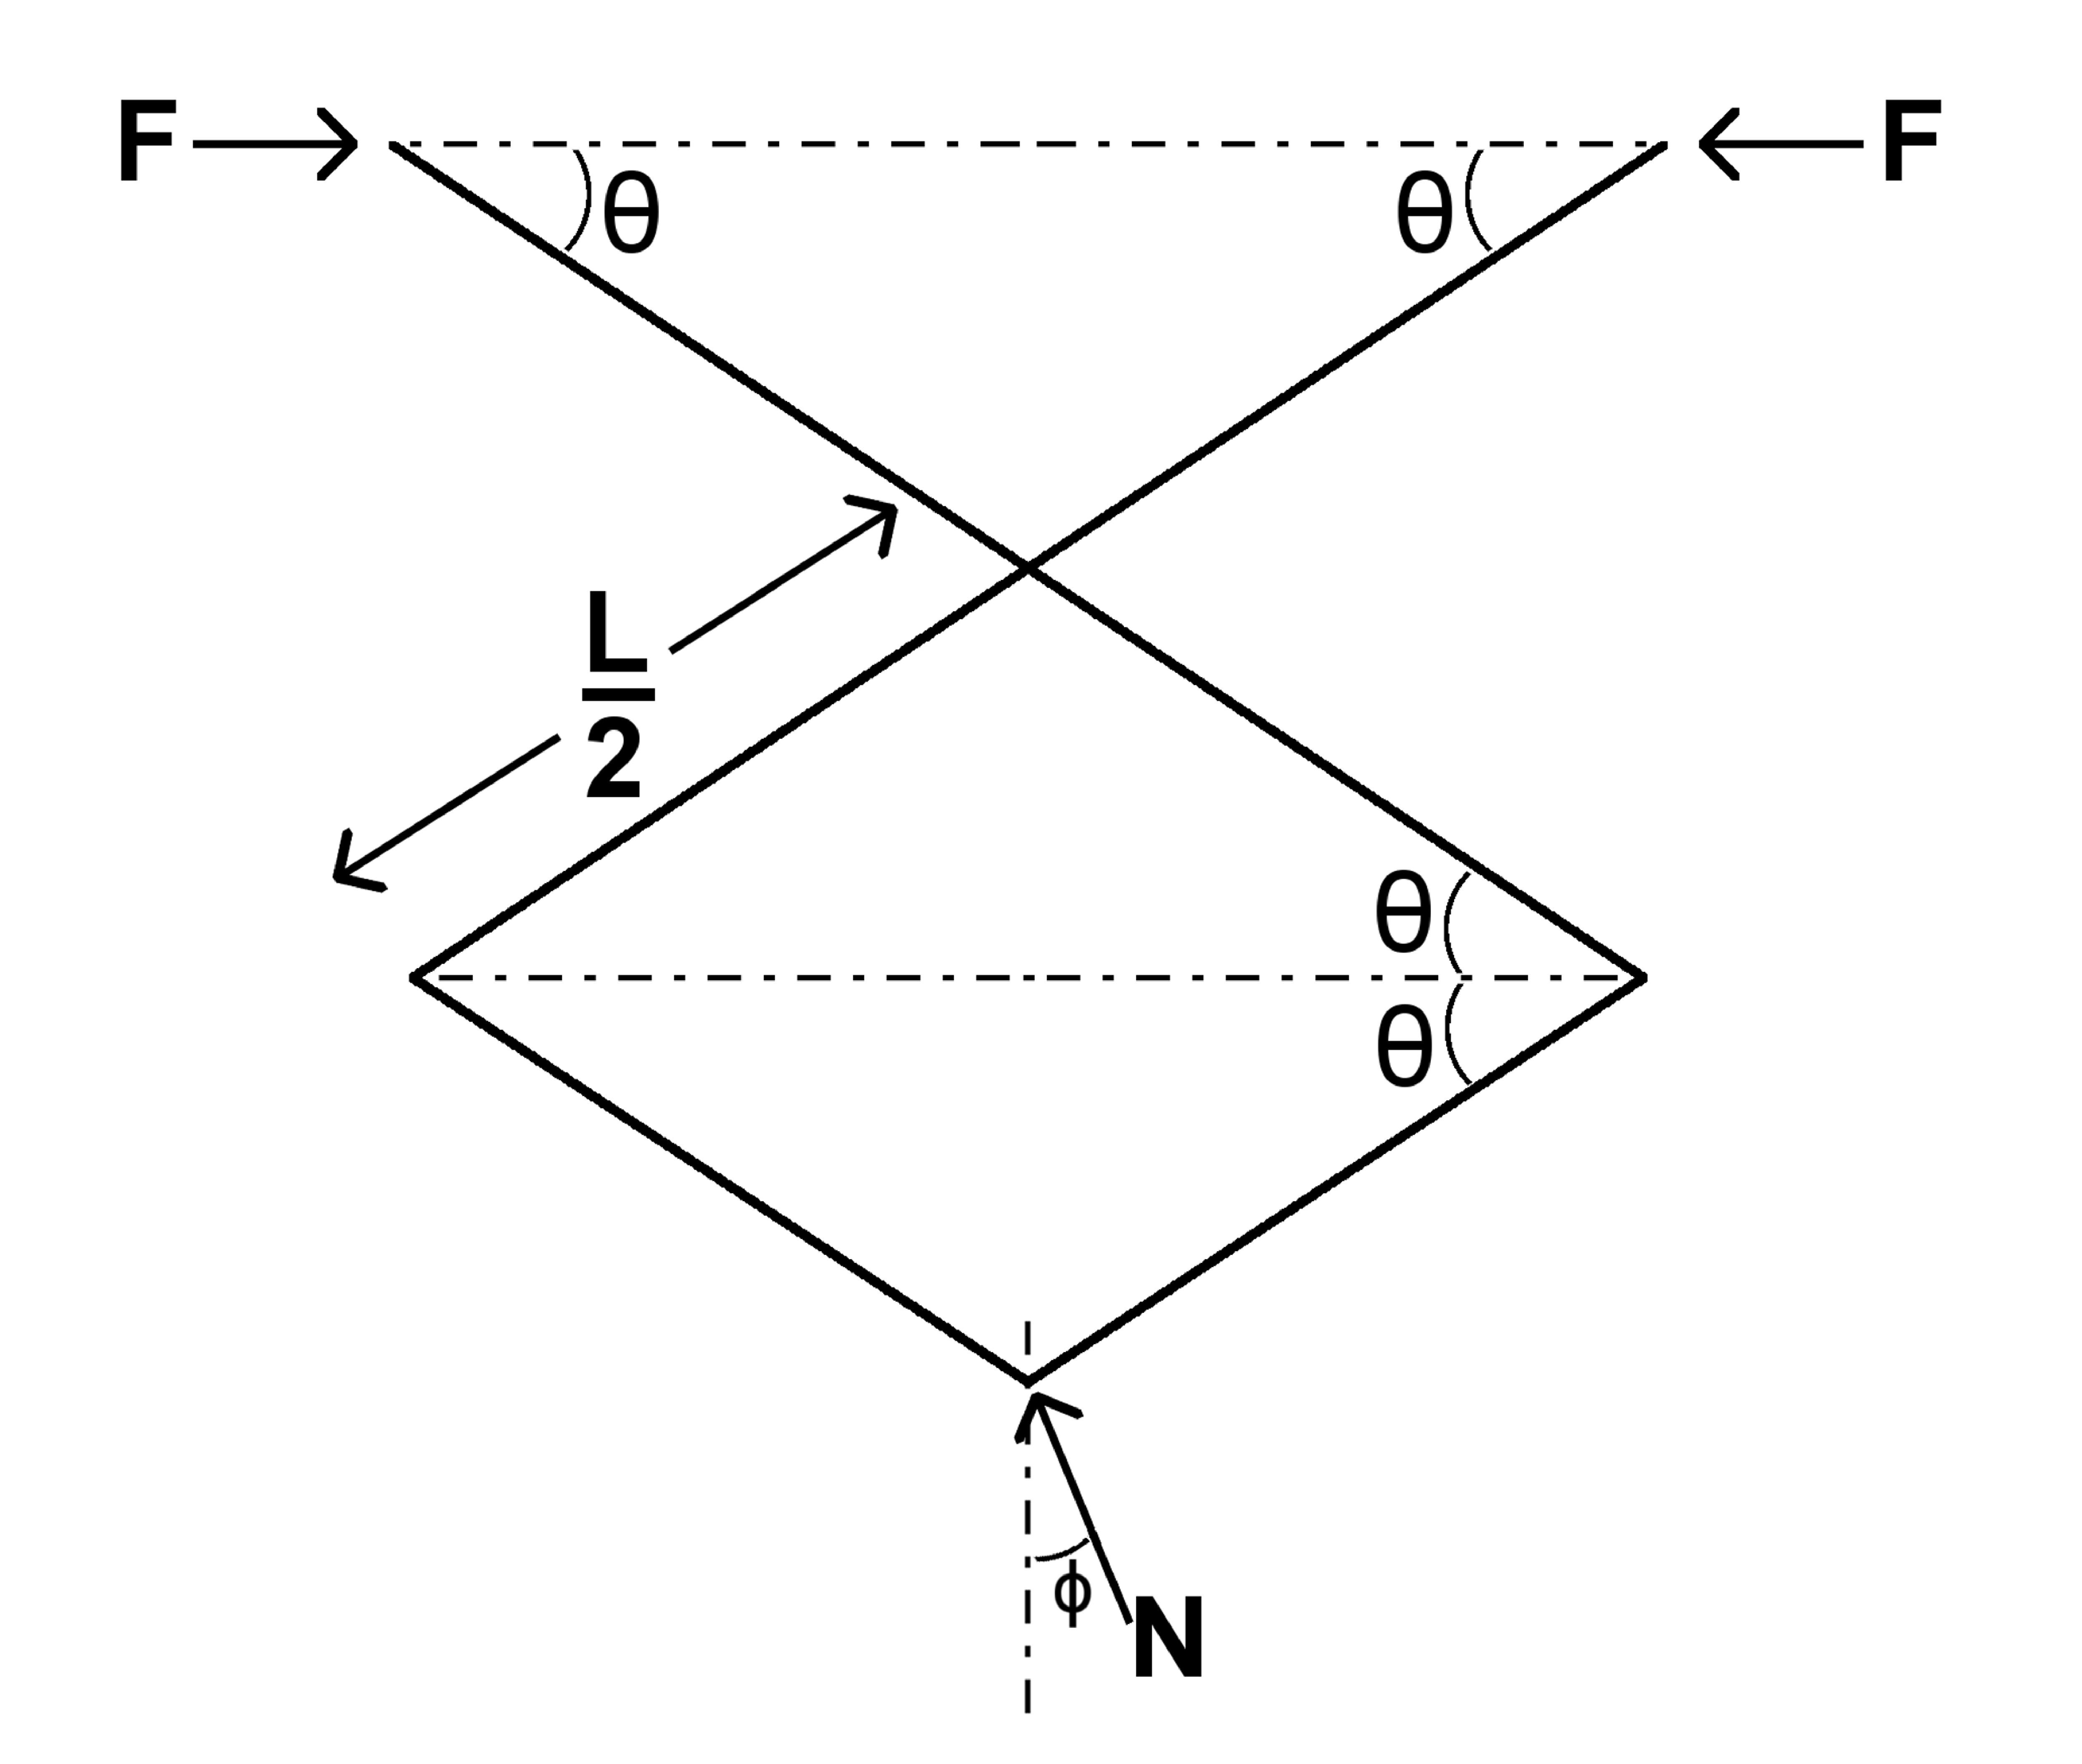
\includegraphics[height=\imageheight]{legDiagram}
					\caption{Labelled Diagram indicating angles referenced in the text}
					\label{legDiagram}
				\end{multicols}
			\end{figure}			
			\begin{figure}[h]
				\centering
				\begin{multicols}{2}
					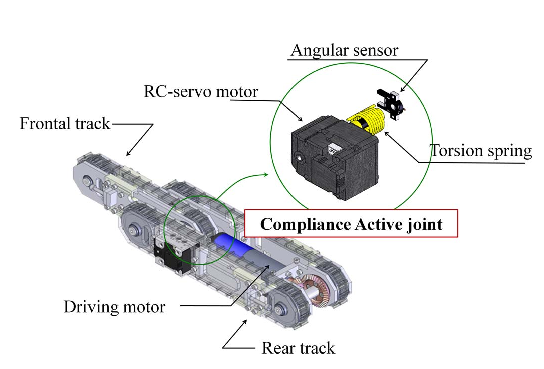
\includegraphics[height=\imageheight]{activeCompliance}
					\caption{Function and construction of an active compliance joint. Figure from \cite{park2010normal}}
					\label{activeCompliance}
					\columnbreak
					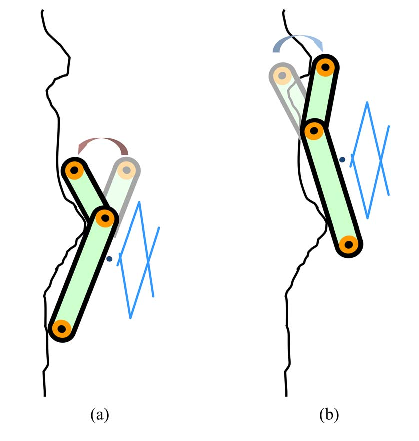
\includegraphics[height=\imageheight]{unevenBehaviour}
					\caption{Behaviour of active compliance joint over uneven surfaces (travelling upwards). Figure from \cite{park2010normal}}
					\label{unevenBehaviour}
				\end{multicols}
			\end{figure}
			\\
			The rotation of the two base legs relative to the body of the robot occurs using a motor to drive each end of the rotation mechanism.
			The motor drives the sun gears of two planetary gear systems, shown in \hyperref[planetaryDrive]{Figure \ref*{planetaryDrive}},which rotate in opposite direction so the legs move symmetrically.
			The direction is reversed for the further planetary drive system using a small differential gearbox, shown in \hyperref[diffGearbox]{Figure \ref*{diffGearbox}}, which allows for compact reversal of motion.
			These allow the legs to move around the body, from almost directly below the robot to in a horizontal plane at $90^\circ$ to the top leg.
			As both legs are driven from the same motor at each end, both legs are symmetrical about the vertical leg at all times, and the leg position can be summarised by a single leg rotation angle $\lambda$, measured from the top leg, which varies from $\lambda = 90^\circ$ to $\lambda = 160^\circ$.
			The rotation allows the robot to adapt to different angles of the pipe more easily, as it will be quicker to drive along horizontal pipes with the almost vertical drive system, whereas vertical pipes require a more even distribution of contact points for optimal behaviour, probably requiring an angle of $\lambda = 120^\circ$ for the most even distribution of contact points.
									
			\begin{figure}[h]
				\centering
				\begin{multicols}{2}
					\includegraphics[height=\imageheight]{planetaryDrive}
					\caption{Planetary drive used to move the legs relative to the main body}
					\label{planetaryDrive}
					\columnbreak
					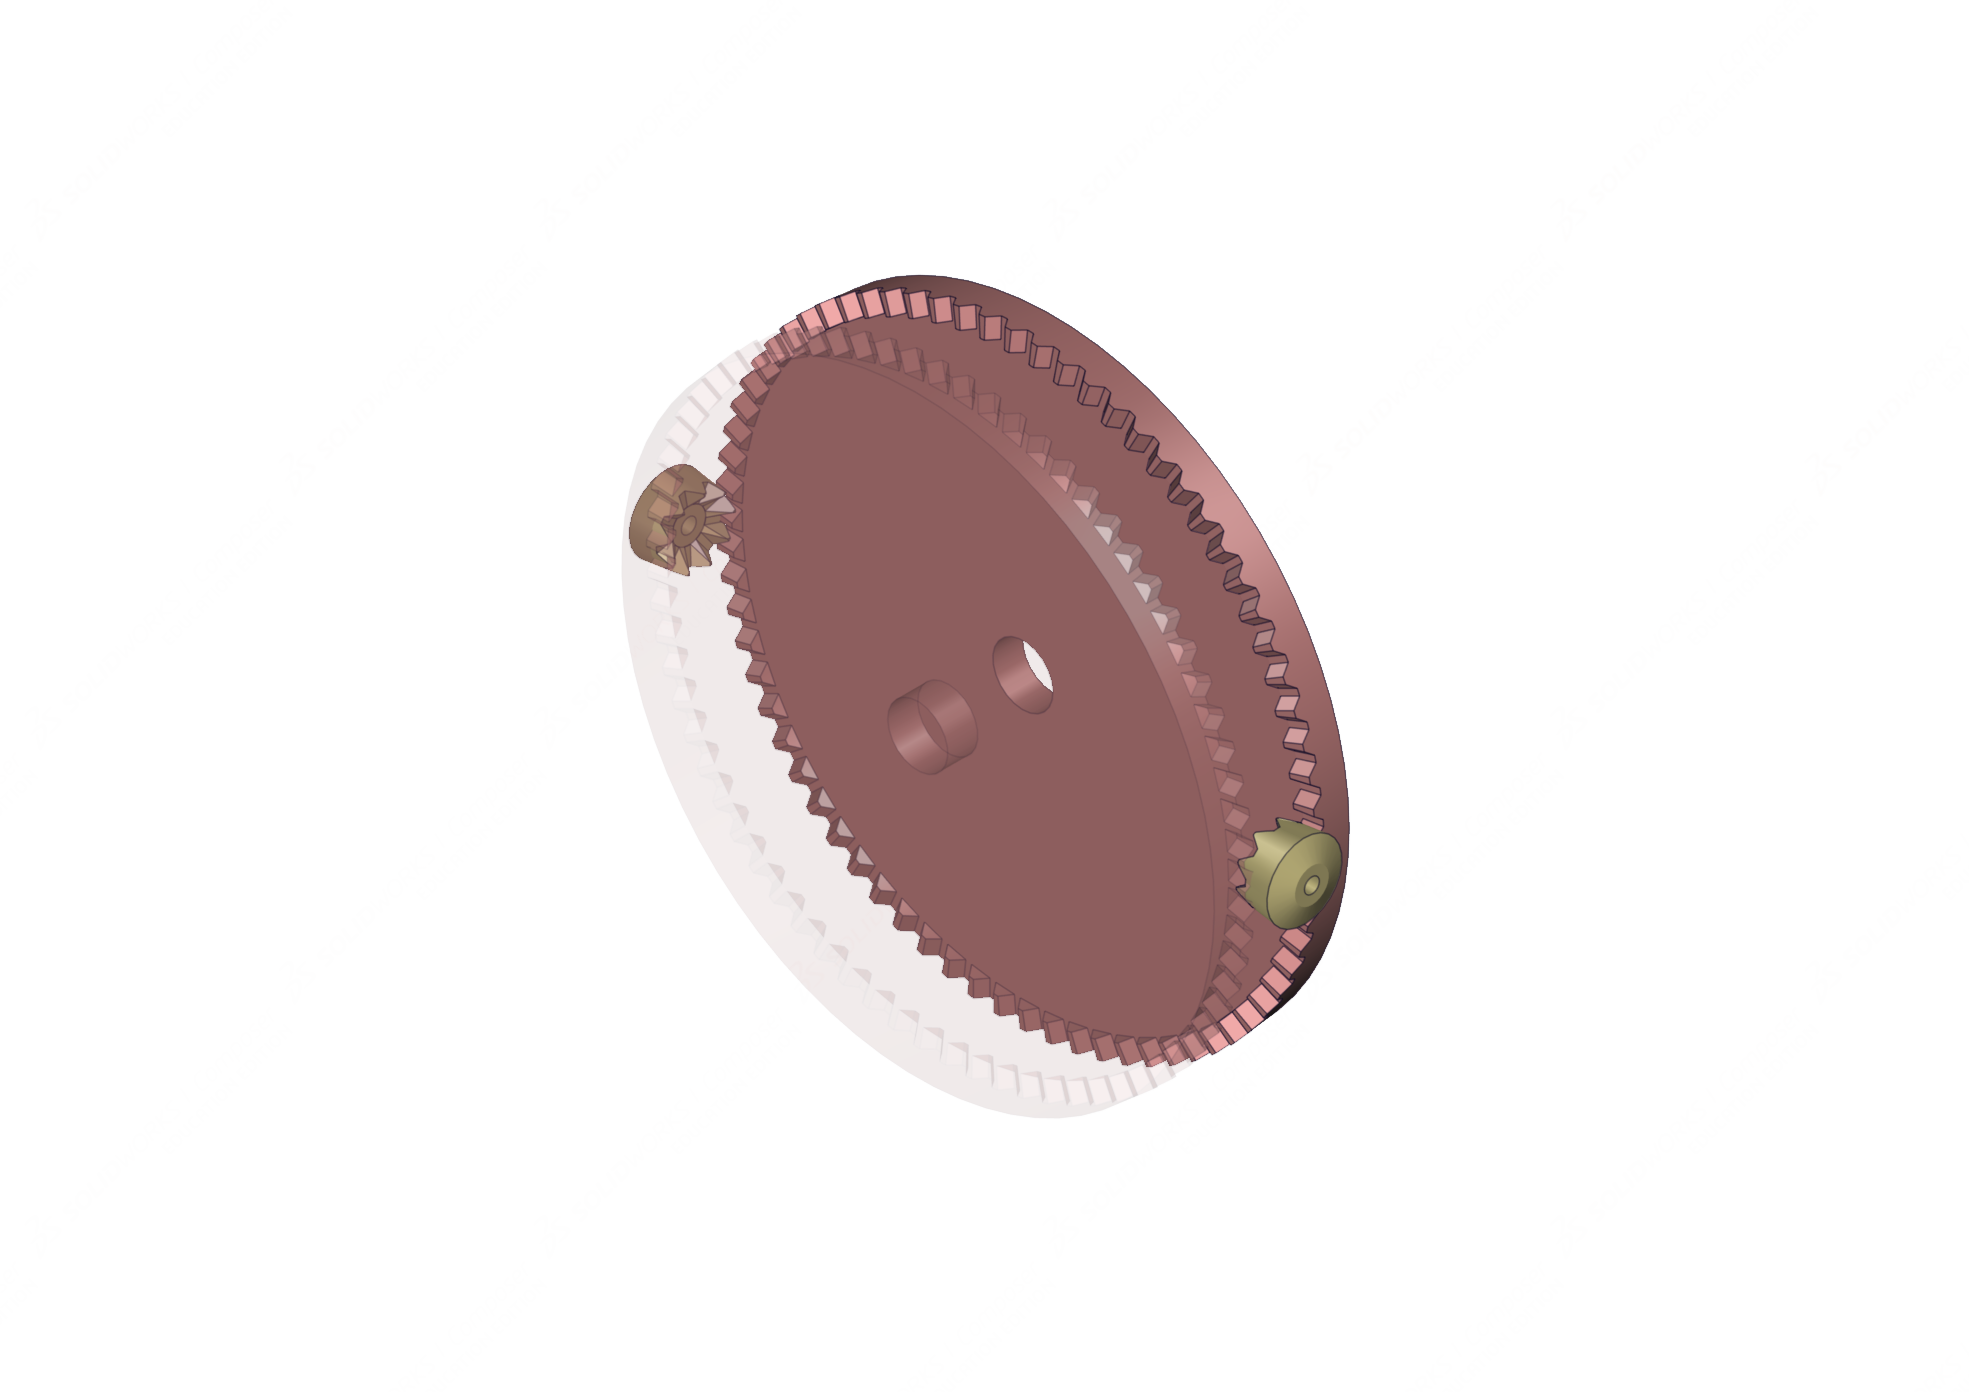
\includegraphics[height=\imageheight]{diffGearbox}
					\caption{Differential gearbox for coaxial rotational direction reversing}
					\label{diffGearbox}
				\end{multicols}
			\end{figure}
			
			The ratio between the longer base links of the pantograph and then shorter tip links is $2:1$, which gives the greatest range of diameters for the smallest change in the base distance\textsuperscript{\cite{okada1987mogrer}}, so we can calculate the required link length $L$ to allow the robot to adapt to the chosen range of diameters, $609.6 - 914.4$ mm.
			The pantograph angles are shown in \hyperref[legDiagram]{Figure \ref*{legDiagram}}, and we can find that:
			
			\begin{align}
				r_{min} &= \frac{3L}{2} \sin \left( \theta_{min} \right)
				\\
				r_{max} &= \frac{3L}{2} \sin \left( \theta_{max} \right)
				\\
				\implies \Delta r &= \frac{3L}{2} \left( \sin \left( \theta_{max} \right) - \sin \left( \theta_{min} \right) \right)
				\\
				L &= \frac{2 \Delta r}{3 \left( \sin \left( \theta_{max} \right) - \sin \left( \theta_{min} \right) \right)}
			\end{align}
			
			If we assume that the pantograph will ideally move from an angle of $\theta_{min} = 20^\circ$ to $\theta_{max} = 60^\circ$, spanning a change in radius of $304.8$ mm, we find that $L = 387.8$ mm, and our smallest leg radius $r_{min} = 199.0$ mm, not including the depth of the tracks.
			This means that, if we assume our track depth is $70$ mm, our body diameter has a maximum of $376.4$ mm, setting a constraint on the dimensions of the inner body based on our design criteria.
			\\
			The minimum length of the body is also set by this, as it means that the body length $l_{min} = L \cos \left( \theta_{min} \right) = 364.4$ mm.
			A maximum body length can be found by considering the ability of the robot to turn corners inside the pipe, and it is necessary to consider how this compares to the minimum to make sure there is no loss of mobility.
			For the duration of this calculation, we will assume we are in the smallest possible pipe diameter $D_{pipe} = 609.6$ mm, and we will assume that the curvature radius $r_c = \frac{3}{2} D_{pipe} = 914.4$ mm.
			As our robot diameter $D_r \nless \left( 2 \sin \left( 45^\circ \right) - 1 \right) D_{pipe} = 252.5$ mm we can use the following equation\textsuperscript{\cite{roh2005differential}}:

			\begin{align}
				l_{max} &= 2 \sqrt{4D_{pipe}^2 - \left( D_{pipe} + D_r\right) ^ 2}
				\intertext{which, using our maximum $D_r = 436.4$ mm}
				l_{max} &= 1252.7 \ \mathrm{mm} \notag
			\end{align}
			% Makes max volume 187*10^6 mm^3
			We can also use \hyperref[legDiagram]{Figure \ref*{legDiagram}} to calculate the required force output of the linear actuators in order for the robot to operate at all angles.
			As such, we consider the worse case scenario, where the robot is climbing vertically, and thus must create enough normal force for friction to support its entire weight.
			We find that:
			
			\begin{align}
				N &= \frac{2 F \tan \left( \theta \right)}{\cos \left( \phi \right)}
				\\
				F_f &= \mu_{t,p} N
				\\
				&= \frac{2 \mu_{t,p} F \tan \left( \theta \right)}{\cos \left( \phi \right)}
				\intertext{where $F_f$ is the frictional force on one track, and $\mu_{t,p}$ is the coefficient of friction between the tracks and the pipe. \newline In order for this to balance the weight W:}
				\begin{split}
					W &= 3 F_f
					\\
					&= \frac{6 \mu_{t,p} F \tan \left( \theta \right)}{\cos \left( \phi \right)} \label{maxWeight}
				\end{split}
				\\
				\implies F &= \frac{W \cos \left( \phi \right)}{6 \mu_{t,p} \tan \left( \theta \right)} \label{reqMaxNorm}
			\end{align}
			
			Since testing would be required to find the greatest angle $\phi$ that is experienced by the robot in general use, as well as an estimate for the coefficient of friction $\mu_{t,p}$, it is tricky to estimate the force required for the actuators.
			However, estimates from other papers for $\mu_{t,p}$,which are $1.21$\textsuperscript{\cite{sato2011development}} - $1.6$\textsuperscript{\cite{park2010normal}}, allow us to create a worst case estimate for the required force of $1.21$.
			From \hyperref[reqMaxNorm]{Equation \ref*{reqMaxNorm}}, we can see that the worst case scenario is with the lowest pipe diameter, as this minimises $\theta$, and we can hypothesise that straight sections, where $\phi$ is expected to be close to $0^\circ$, will require the most linear actuator force.
							
		\subsection{Power}
		
		\subsection{Sensing}
		
		\subsection[Communications]{Communications - Louis Emmanuel}
		%by Louis

		Communication is an important capability for the autonomous robot as in order to operate it safely and efficiently, it's critical to know the whereabouts of the robot within the pipe at any given time. An additional and more complex requirement is also the ability for bidirectional communication so the robot can be updated on its position and given instructions when necessary. 
		\\
	    The difficulty arises in finding a suitable communication method that is capable of operating in the difficult pipeline environment. With pipe bends, thick steel walls, metres of soil, and noise interference, the choice of communication must be able to overcome these barriers without inhibiting locomotion. Figure 8 outlines several communication methods which have been widely practiced in the Oil and Gas industry\textsuperscript{\cite{acoustic2020}}.
	    \\
         A critical requirement of the robot is for it to have a real time understanding of its location in order to navigate pipes and localise pipe damage. From the solutions in Figure 8, the only methods capable of this are ELF and wiring. However, ELF communications requires a significantly sized receiver [6] which is infeasible to house in the robot without inhibiting speed, locomotion and range. Consequently, for feeding data to the robot, a wire will be used.\\ 
         \hspace*{3ex}Although a wire allows bidirectional communication, it is incapable of determining the position of the robot. Therefore, a method of communicating with surface receivers must be used in order to determine its position. Given the size constraints and interference challenges, acoustic and magnetic methods are unsuitable for this application. Instead, ELF communication is used which with present technology [x] is capable of traveling through up to 20m of soil. This allows location to be determined, and fed back to the robot through the wiring in order to compensate for the the accumulated locating error generated in the on board INS.
         
        $\textbf{Communication Map}$
        
        \begin{figure}[h]
			\centering
			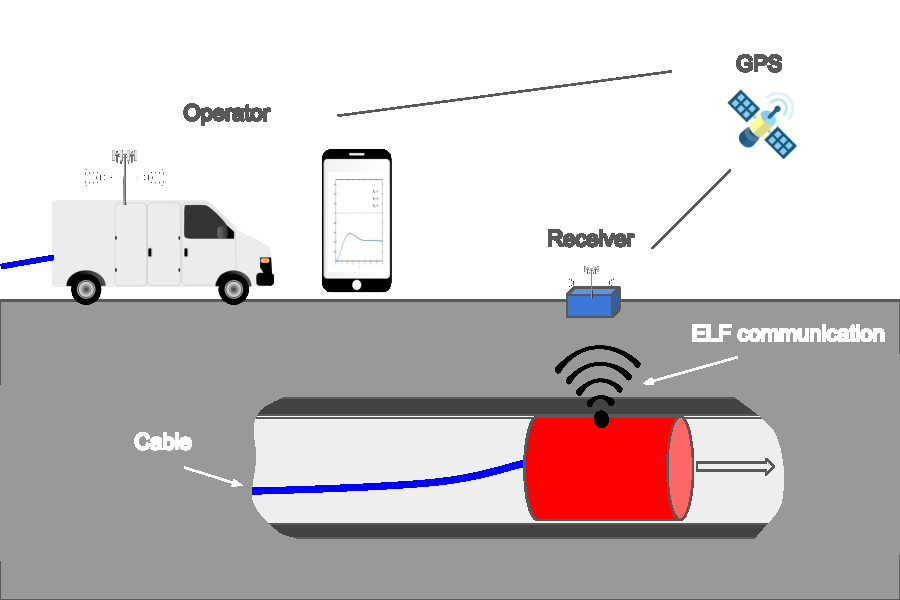
\includegraphics[scale=1]{comms layout.pdf}
			\caption{Communications layout}
			\label{comparison comms}
		\end{figure}
        
        Figure 9 provides an overview of the communication architecture. Starting from the operator, an optical fibre which is capable of bidirectional communication is fed down to the robot by an automatic cable reel. On board the robot is an ELF transmitter which pulses ELF waves at 22Hz to to the receivers above ground. These receivers then calculate the global position of the robot, and feed it back down to the robot via the optical fibre.
       
        \textbf{Wired connection}\\
        The wired communication line presents a challenge for the locomotion of the robot. In order to satisfy the communication requirements, it must deliver data at a suitable rate without creating a hindrance to locomotion along the pipe and around corners. The proposed solution uses a kevlar lined wire with an optical fibre. 
        Through making assumptions on a constant frictional coefficient throughout the pipe and steady speed, we arrive at the following initial equation for drag. 
        \begin{align}
				F_0 = \mu_g L_{wire}   g \rho
		\end{align}
        
        % Not sure about this value of F0
        
        Where $L_{wire}$ is the length of wire at current time, $\mu_g$ is the coefficient of friction between the cable and ground and $\rho$ is the mass per unit length of the cable.
        
        This equation is very simple and does not take into account the corners our robot is designed to navigate. Therefore, through modelling corners as segments of a cylinder, we can justify the use of the capstan equation [x] which describes the resistance to sliding of a flexible but inextensible cord wrapped around a cylinder. For a series of corners, the following equation is derived.
        \begin{align}
                F_D = F_0 \boldsymbol{\cdot} {e}^{\mu_c \sum \alpha}
        \end{align}

		Where $\mu_c$ is the coefficient of friction between the cable and corners and $\alpha$ is the angle swept by the cable around the cylinder in radians. 
	    Hence, in order to minimise this drag force, a solution must be found that satisfies our bandwidth capabilities whilst minimising the mass per length and friction coefficients.  
	    In this case, a Fiber optic cable is better in almost every sense over alternatives. For example, a typical fiber cable weighs 4Lbs/1000ft, requires a power of 2W and is immune to noise. In comparison, the next best alternative is copper wire which weighs 36Lbs/1000ft, requires >10W of power and is susceptible to EM interference [x]. \\

	    Finally, in order to minimise friction coefficients and absorb the large tensile strength in the wire, a protective coating must be applied to the cable. This technology is widely developed with smoothed Kevlar reinforced cable offering a low friction coefficient whilst resisting tensile strengths up to 2800MPa [x]. For the case of a 5mm Kevlar reinforced optical fibre cable, a breaking force of 54kN can be achieved. Considering an upper estimate of Equation 12 using $\mu$ = 0.2 [x] L = 500m $\rho$ = 0.04 $Kgm^-1$ [x] $\sum \alpha = 10\pi/2$, a tensile force of $F_D$ = 907N is estimated which is well below maximum. 
	    
	    \textbf{Automatic Cable Reel}

        From Equation 12, it is demonstrated that the drag force on the robot is directly proportional to the length of wire. Therefore, a requirement for the reel is for it to supply the minimum amount of wire without introducing significant tension. Further, the reel must be capable of self winding when the robot makes its return journey, otherwise it will impede it.\\ 
        \hspace*{3ex}Fortunately there are established solutions which provide this capability. The automatic cable reels offered by Minicam and IPEK both offer motorised winding which is specialised for robot pipe inspection. 
        Figure 10 compares the weight, size, power consumption and cost of each solution. The MiniCam ACR 500 is chosen as it is lighter and smaller. 


        
        %INSERT QUOTE PRICE
        \begin{figure}[h]
			\centering
			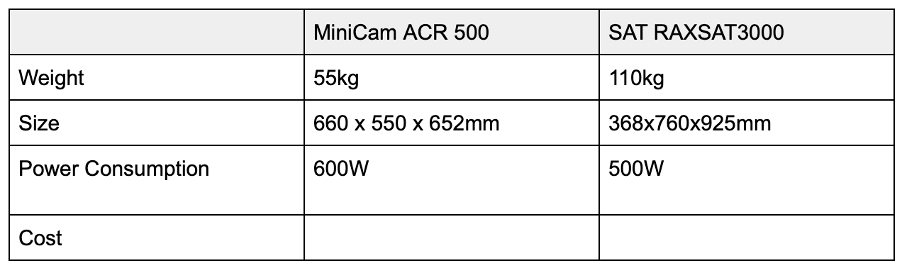
\includegraphics[scale=1]{cablereel.png}
			\caption{Comparison of Existing Cable Reel solutions}
			\label{comparison comms}
		\end{figure}
        







        \textbf{ELF transmitter and Receiver:}
        

		
		
		
		
		\subsection{External Hardware}
		
		% Launch Tube
		
		% Beacons - maybe comms?
	
		\subsection{Materials \& Construction}
		
		% TBD after 14/2/21 - needs pressure force calcs etc
	
	\section{Software}
		
		\subsection[Inclination Detection]{Inclination Detection - Jim Laney}
		
		The robot is able to detect the inclination of the pipe it is in for calculation of the required leg force, as well as to aid in the mapping of the pipe.
		While the AHRS can give the angle of the robot relative to the wider world, it is not guaranteed that the robot body is parallel to the pipe.
		As such, the angle between the pipe and the robot needs to be accounted for in order to correctly measure the pipe angle.
		\\
		\begin{figure}[h]
			\centering
			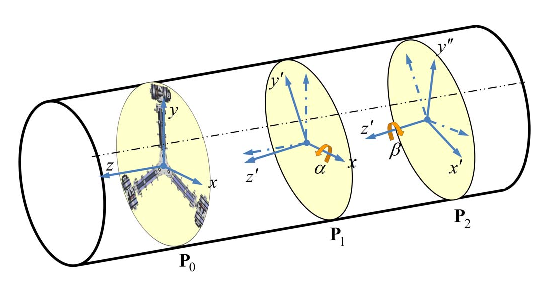
\includegraphics[height=\imageheight]{pipeOrientation}
			\caption{Angles used for calculation of pipe angle. Figure from \cite{park2010normal}}
			\label{pipeOrientation}
		\end{figure}
		\begin{figure}[h]
			\centering
			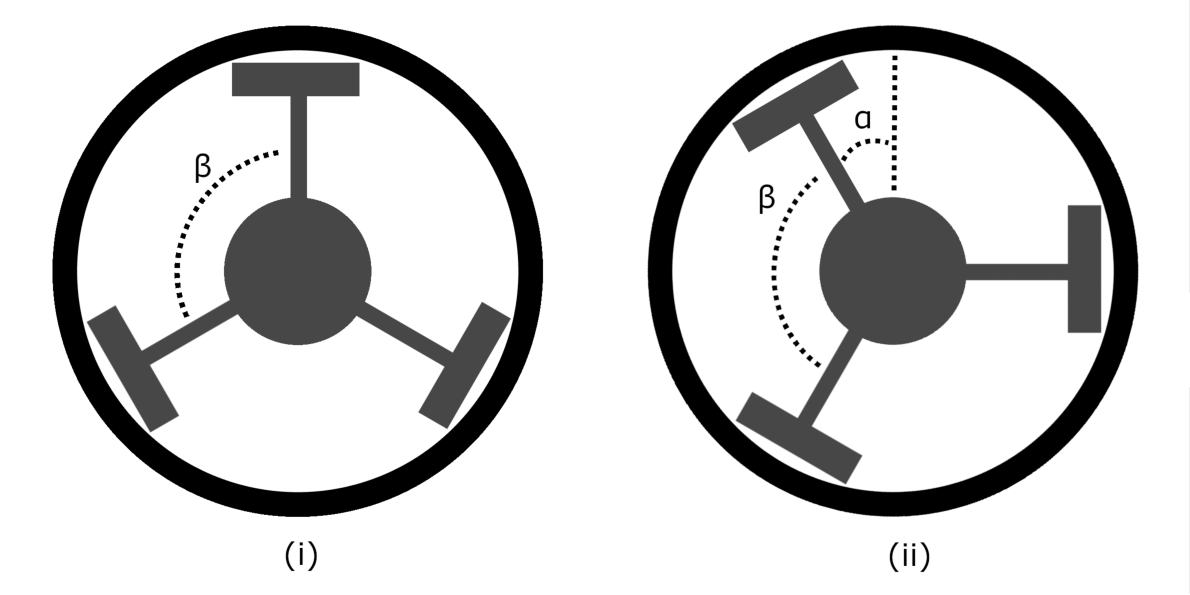
\includegraphics[height=\imageheight]{pipeAngle}
			\caption{Position of the robot within the pipe. (i) Within a horizontal or vertical bend, (ii) Within a bend at angle $\xi$ to the vertical, view shown relative to the bend rather than relative to the outside world}
			\label{pipeAngle}
		\end{figure}
		As in \hyperref[pipeOrientation]{Figure \ref*{pipeOrientation}}, the angle of the robot within the pipe can be decomposed into two orthogonal rotations, of $\alpha$ about the pipe diameter, and then $\beta$ about the robot centre, shown as $z'$ in the figure.
		Since the angle of the top leg, $\phi_T$, is $\alpha$ on the $y'$ axis ($\beta = 0$), but zero on the x axis ($\beta = 90^\circ$), we can estimate our angle using:
		\begin{align}
			\phi_T &= \cos \left( \beta \right) \alpha
			\\
			\phi_L &= \cos \left( \beta + \lambda \right) \alpha
			\intertext{where $\lambda$ is the leg rotation angle as shown in \hyperref[pipeAngle]{Figure \ref*{pipeAngle}}:}
			\frac{\phi_L}{\phi_T} &= \frac{\cos \left( \beta + \lambda \right)}{\cos \left( \beta \right)}
			\\
			\beta &= \tan^{-1} \left( \frac{1}{ \sin \left( \lambda \right)} \left( \frac{\phi_L}{\phi_T} + \cos \left( \lambda \right) \right) \right)
			\\
			\alpha &= \frac{\phi_T}{\cos \left( \beta \right)}
		\end{align}
		Once we have found the individual rotations of the robot, we can combine this with the AHRS data to find the pipe angle relative to the outside world.
		\\
		Since we are working in 3D we assume that the AHRS returns rotations in a matrix $\mathbf{R}_{R,W}$, which gives the angle of the robot relative to the world.
		We want to find $\mathbf{R}_{P,W}$, the rotation of the pipe relative to the world, so we create a matrix $\mathbf{R}_{P,R}$ which gives the rotations of the pipe, relative to the robot:
		\begin{align}
			\mathbf{R}_{P,R} &=
			\begin{bmatrix}
				\cos \left( \alpha \right) & 0 & - \sin \left( \alpha \right)
				\\
				- \sin \left( \alpha \right) \sin \left( \beta \right) & \cos \left( \beta \right) & - \cos \left( \alpha \right) \sin \left( \beta \right)
				\\
				\sin \left( \alpha \right) \cos \left( \beta \right) & \sin \left( \beta \right) & \cos \left( \alpha \right) \cos \left( \beta \right)
			\end{bmatrix}
			% Matrices can be shrunk using smallmatrix rather than bmatrix but for now no need to - smallmatrix requires you to pu \left[ and \right] on either side of the smallmatrix environment
			\\
			\mathbf{R}_{P,W} &= \mathbf{R}_{P,R} \ \mathbf{R}_{R,W}
			\intertext{We then use the general form of a rotation matrix to determine the yaw, roll and pitch from $\mathbf{R}_{P,W}$:}
			\mathbf{R}_{P,W} &= \left[
			\begin{smallmatrix}
				\cos(\psi_x) \cos(\psi_y) & \quad & \sin(\psi_x) \cos(\psi_y) \sin(\psi_z) - \sin(\psi_y) \cos(\psi_z) & \quad & \sin(\psi_x) \cos(\psi_y) \cos(\psi_z) + \sin(\psi_y) \sin(\psi_z)
				\\
				\\
				\cos(\psi_x) \sin(\psi_y) & \quad & \sin(\psi_x) \sin(\psi_y) \sin(\psi_z) + \cos(\psi_y) \cos(\psi_z) & \quad & \sin(\psi_x) \sin(\psi_y) \cos(\psi_z) - \cos(\psi_y) \sin(\psi_z)
				\\
				\\
				- \sin(\psi_x) & \quad & \cos(\psi_x) \sin(\psi_z) & \quad & \cos(\psi_x) \cos(\psi_z)
			\end{smallmatrix} 
			\right] \notag
			\\
			\psi_x &= \sin^{-1} \left( \ \mathbf{R}_{P,W} \left[ 3, 1\right] \ \right) \label{pipeX}
			\\
			\psi_y &= \tan^{-1} \left( \frac{\ \mathbf{R}_{P,W} \left[ 2, 1\right] \ }{\mathbf{R}_{P,W} \left[ 1, 1\right]} \right) \label{pipeY}
			\\
			\psi_z &= \tan^{-1} \left( \frac{ \ \mathbf{R}_{P,W} \left[ 3,2 \right] \ }{\mathbf{R}_{P,W} \left[ 3,3 \right] } \right) \label{pipeZ}
		\end{align}
		Thus, in order to increase the efficiency of the algorithm, we only need to calculate the relevant entries of $\mathbf{R}_{P,W}$, meaning that the number of computations required can be reduced to $\frac{5}{9}$ of the original value.
		These angles can also be used to help with the identification of other things within the robot, but the reliability of these is not guaranteed, as the angle of the legs can be affected by other factors, such as unevenness in the pipe wall.
		As such, the value for the inclination of the pipe should be averaged out to give better results for pipe inclination, and giving a smoother projection of the map overall.
		
		\subsection[Leg Actuation Control]{Leg Actuation Control - Jim Laney}
		
		The robot needs to be able to accurately control the length of its legs in order to maintain the correct normal force for operation.
		We know the required linear actuator force for climbing vertically from \hyperref[reqMaxNorm]{Equation \ref*{reqMaxNorm}}, which we can modify to find that:
	
		\begin{align}
			F &= \frac{W \sin \left( \psi_x \right) \cos \left( \phi \right)}{6 \mu_{t,p} \tan \left( \theta \right)} \label{idealForce}
		\end{align}
	
		where $\psi_x$ is the inclination of pipe in the vertical plane, worked out from \hyperref[pipeX]{Equation \ref*{pipeX}}.
		\\
		However, when the pipe inclination is zero - i.e we are travelling in a horizontal direction - \hyperref[idealForce]{Equation \ref*{idealForce}} breaks down and the required force $F$ becomes $0$.
		The required normal force when travelling in the horizontal pipe is the weight $W$.
		Thus our new equation for the normal force:
		\begin{align}
			\begin{split}
				N &= \left( N_{max} - W \right) \sin \left( \psi_x \right) + W
				\\
				&= \frac{2 F \tan \left( \theta \right)}{\cos \left( \phi \right)}	
			\end{split}
			\\
			N_{max} &= \frac{W}{3 \mu_{t,p}}
			\\
			\implies \frac{2 F \tan \left( \theta \right)}{\cos \left( \phi \right)} &= W \sin \left( \psi_x \right) \left( \frac{1}{3 \mu_{t,p}} - 1 \right)  + W
			\intertext{Thus our equation for $F$ becomes:}
			F &= \frac{ W \cos \left( \phi \right)}{ 2 \tan \left( \theta \right) } \left( \sin \left( \psi_x \right) \left( \frac{1}{3 \mu_{t,p}} - 1 \right) + 1 \right)
		\end{align}
		\\
		Thus, if we know the weight of the robot, and we can estimate the pipe inclination $\psi_x$, as well as measuring the leg and foot angles $ \theta \ \& \ \phi$, we can estimate the required actuator force.
		This means that the robot can set a target actuator force at all times in order to ensure that it able to traverse the pipe.
		\\
		While we initially considered having sensors on the robot to work out the pipe diameter, a much simpler solution was to use the linear actuators themselves. 
		Since we know the required normal force, we can extend the actuators, updating our value of theta until we reach that force, or close to it, using a $H_{\infty}$ controller.
		Thus, the force can be controlled to the point where the target value is reached, and the pipe diameter can be estimated by finding the base angle $\theta$.
	
		\begin{align}
			\cos \left( \theta \right) &= \cos \left( \theta_{min} \right) + \frac{E}{L}
			\intertext{where E is the extension of a single actuator. \newline We can then find that}
			D_{pipe} &= D_r + \frac{3 L}{2} \sin \left( \cos ^{-1} \left( \theta \right) \right)
			\\
			&= D_r + \frac{3 L}{2} \sin \left( \cos ^{-1} \left( \cos \left( \theta_{min} \right) + \frac{E}{L} \right) \right)
		\end{align}
	
		\hyperref[legDiagram]{Figure \ref*{legDiagram}} is reproduced as \hyperref[legDiagramRep]{Figure \ref*{legDiagramRep}} for reference of variables used.
		\\
	
		\begin{figure}[h]
			\centering
			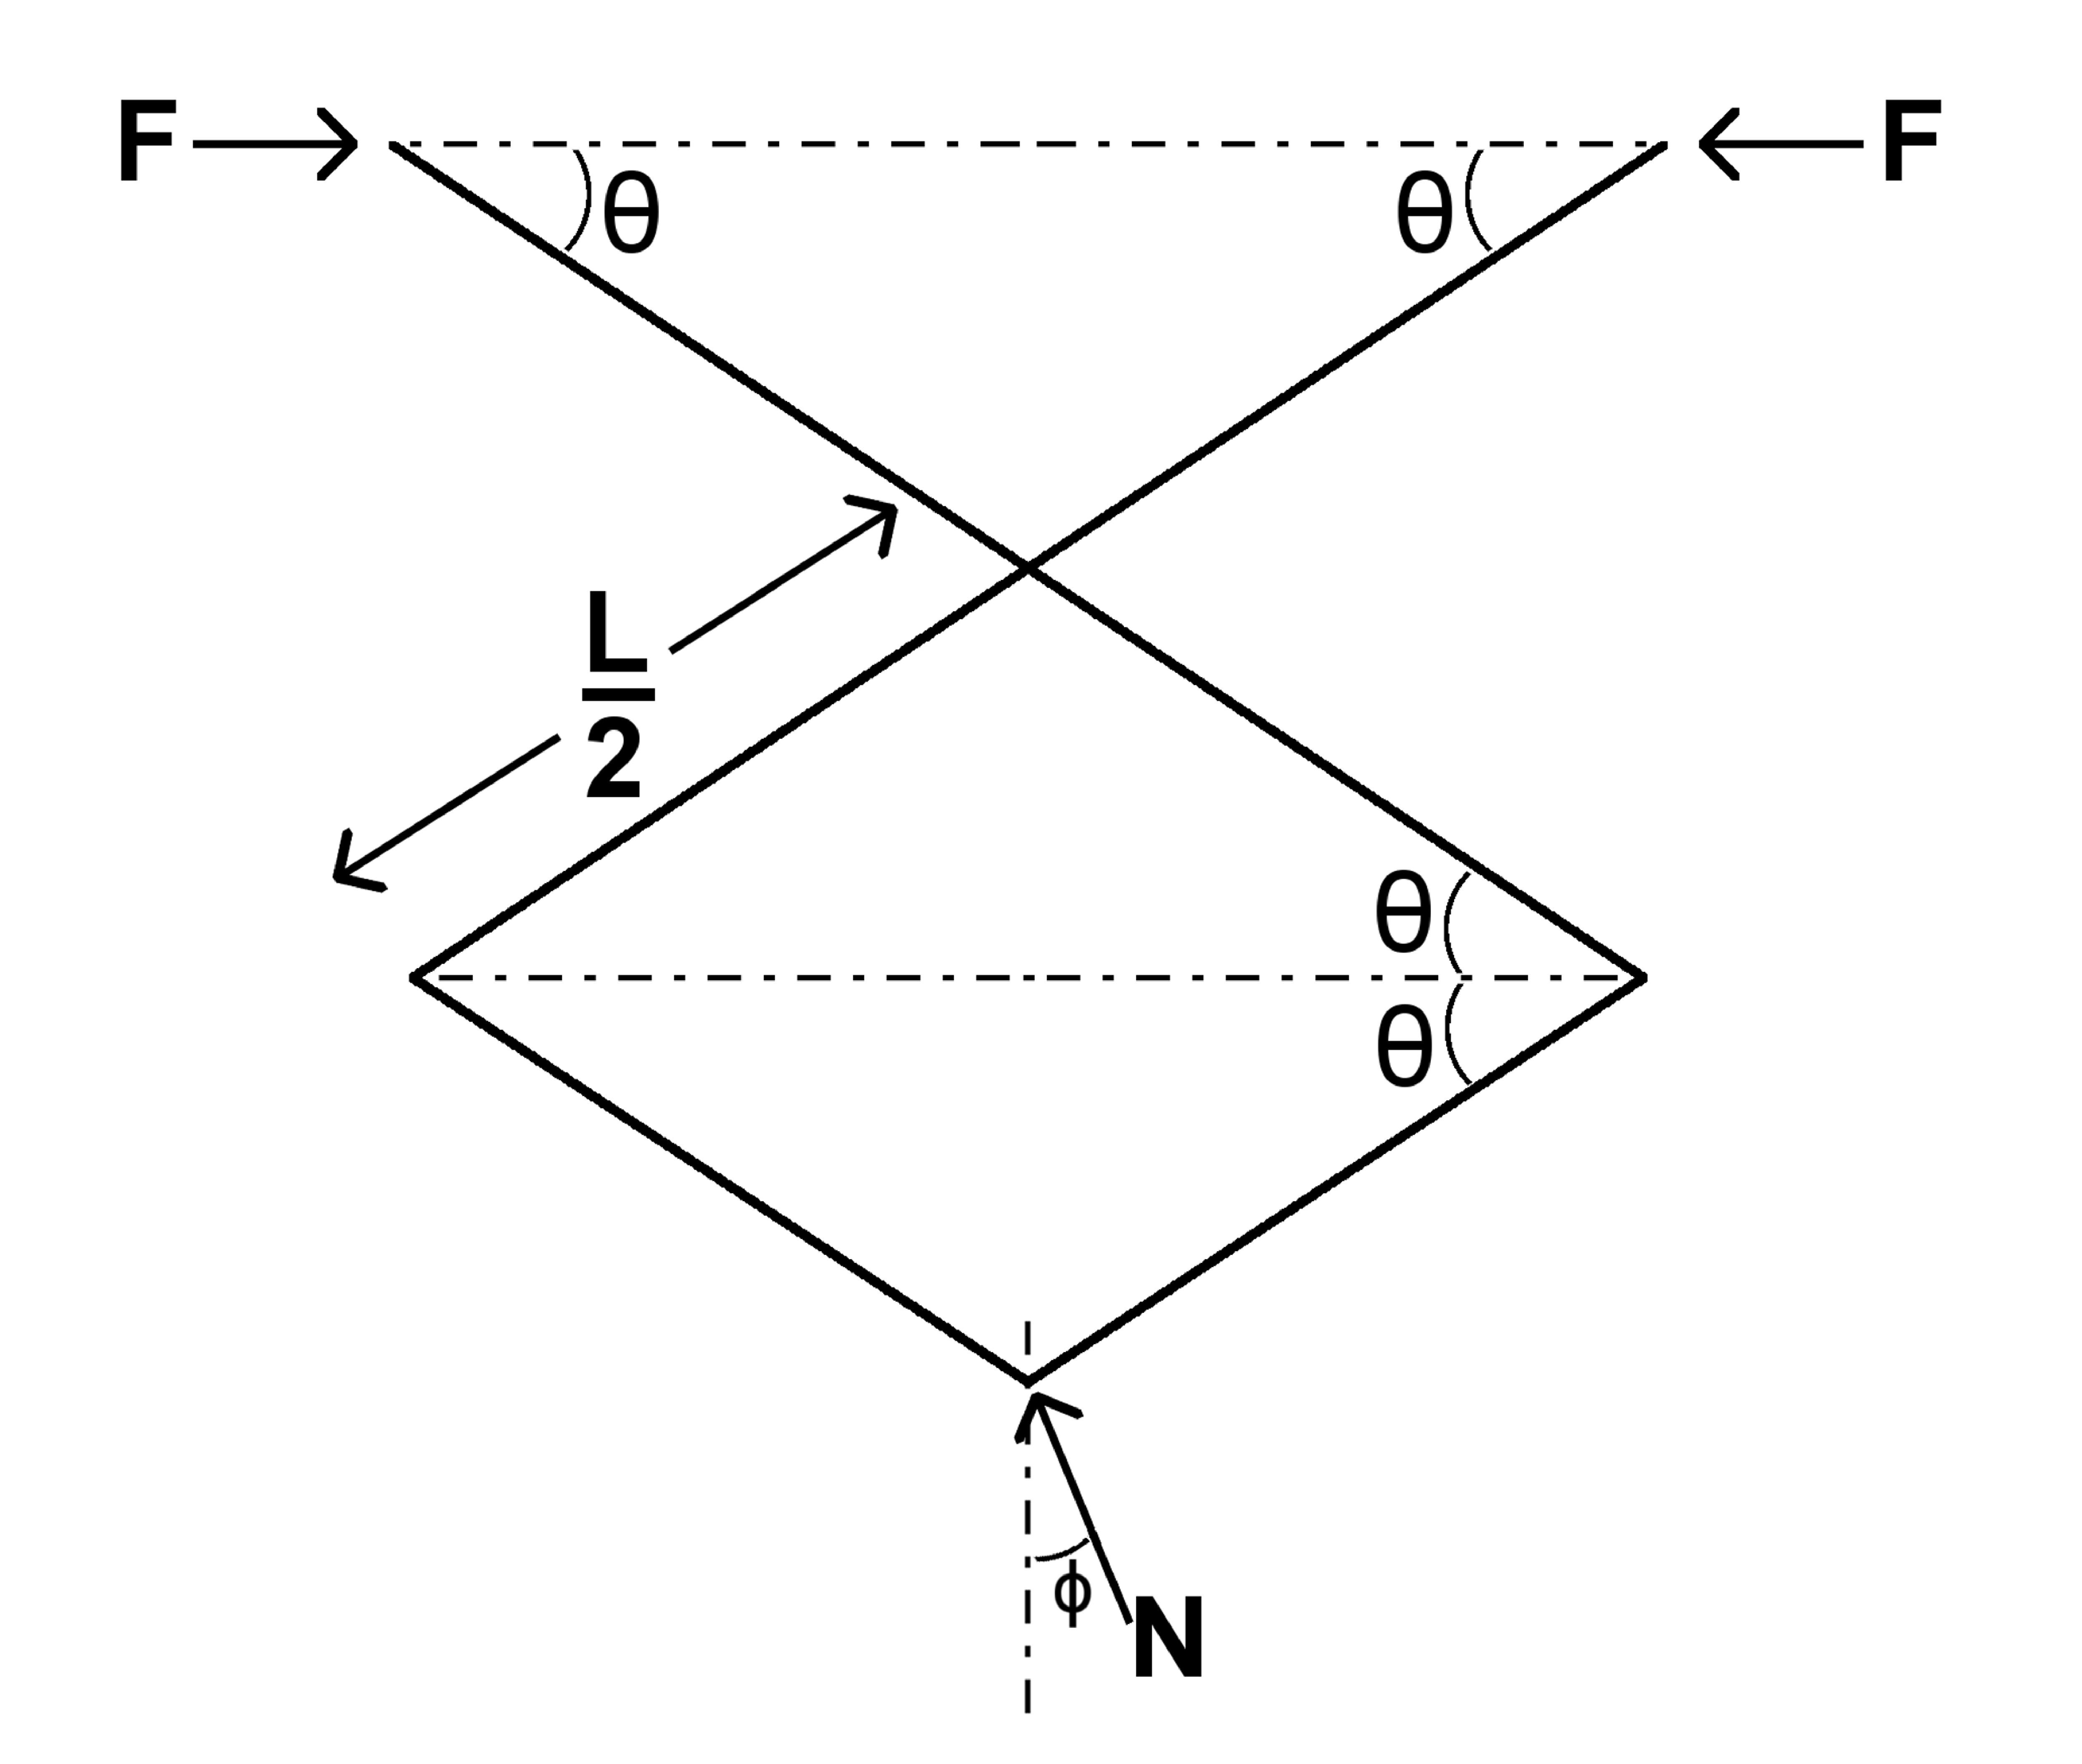
\includegraphics[height=\imageheight]{legDiagram}
			\captionsetup{list=no}
			\caption{Labelled Diagram indicating angles referenced in the text}
			\label{legDiagramRep}			
		\end{figure}
	
		 $H_{\infty}$ control was chosen as the system dynamics can be well modelled for the extension of the leg, and fast performance is required.
		 This is because too little normal force is possible catastrophic, if the robot is travelling up a steeply inclined pipe, and too much normal force for too long could damage critical components.
		 While the system is non-linear, most of the variables simply contribute as fixed values, with the system only being non-linear in $\theta$.
		 However, in the region $20^\circ - 60^\circ, \sin \left( \theta \right)$ is relatively linear, so a linear control method was chosen.
		
		\subsection[Bend Behaviour]{Bend Behaviour - Jim Laney}
		
		The robot requires knowledge of where it is in the pipe, and being able to calculate the position of bends in the pipe is important.
		The robot is designed to travel around bends autonomously, and then report back to the mapping software that it has turned a bend, as well as calculating the angle turned through.
		When turning a bend, the robot uses angular encoders at the end of each leg to tell the individual leg bends $\phi_T$, $\phi_L$ \& $\phi_R$.
		These are detected from angular encoders connected to each leg link which are averaged, so $\phi_L = \frac{\phi_{L1} + \phi_{L2}}{2}$ and equivalent for the other legs.
		The robot can then vary the speed of the tracks at the end of each leg in order to try and get the angles to be parallel, such that $\phi_L = \phi_R = \phi_T$.
		This is done by setting the top leg angle $\phi_T$ as a reference, and controlling the speed using the difference between this and $\phi_R$ or $\phi_L$ with a PID controller.
		This controller only needs a very low natural frequency, as faster changes in the angle are probably due to surface unevenness, which should be dealt with by the active compliance joint.
		\\
		The robot is able to estimate the magnitude of the bend angle based on the distance travelled and the pipe diameter.
		If the bend is in the horizontal plane, as shown in \hyperref[pipeAngle]{Figure \ref*{pipeAngle}(i)}, the robot has to look at the differences between the non vertical legs in order to determine bend angles and directions.
		The robot integrates the speed of each track over the travel of the robot in order to determine the distance travelled.
		When there is disparity between the measured distance by each of the legs, but all tracks are travelling at the same speed, it can be concluded that a bend has been turned, and the robot is again travelling straight.
		Once the bend angle has been determined, this difference can be subtracted in order to realign the values of the track distances covered so that future bends can be identified.
		The inclination calculation also returns the angle of the pipe, which can be used to check the calculations, and ensure that the signs of the calculated bends are correct.
		\\
		If the leg rotation angle $\lambda = 90^\circ$, so that the side legs form a plane across the diameter of the pipe, the angle change can simply be found by using
		\begin{align}
			d_{inner} &= \theta_{bend} \left( r_c  - \frac{ D_{pipe} }{2} \right)
			\\
			d_{outer} &= \theta_{bend} \left( r_c  + \frac{ D_{pipe} }{2} \right)
			\\
			\implies \Delta d &= \theta_{bend} D_{pipe}
		\end{align}
		where d is the distance calculated from the integration of the track speed.
		\\
		The robot legs are typically not going to be in this position, so instead the value of $\lambda$ needs to be factored in, which can be achieved by adjusting the effective pipe diameter:
		\begin{align}
			D_{eff} &= D_{pipe} \sin \left( \lambda \right)
			\\
			\Delta d &= \theta_{bend} D_{eff}
			\\
			\Delta d &= \theta_{bend} D_{pipe} \sin \left( \lambda \right)
			\intertext{Thus the bend angle in the horizontal plane can be caluclated as}
			\theta_{bend} &= \frac{d_{left} - d_{right}}{D_{pipe} \sin \left( \lambda \right)}
		\end{align}
		This means that the angle $\lambda$ cannot be $180^\circ$, since this would result in the angle being incalculable, since there is no differential between the two rotating tracks.
		However, this position is obviously not possible, as the tracks cannot occupy the same space, and thus there will always be a differential to calculate the bend angle over.
		\\
		If the bend is instead in the vertical plane, also shown as \hyperref[pipeAngle]{Figure \ref*{pipeAngle}(i)}, only the top leg's distance will be different, as the two side legs should be moving around an equally long path.
		The bend angle can thus be found by comparing the distance of the outer leg with the distance of the side legs, which must again be adjusted for $\lambda$.
		Assuming an upwards bend:
		\begin{align}
			d_{top} &= \theta_{bend} \left( r_c  - \frac{ D_{pipe} }{2} \right)
			\\
			d_{side} &= \theta_{bend} \left( r_c + \frac{D_{pipe} \cos \left( \lambda \right)} {2} \right)
			\\
			\Delta d &= \theta_{bend} \frac{ D_{pipe} \left( 1 + \cos \left( \lambda \right) \right)}{2}
			\\
			\implies \theta_{bend} &= \frac{2 \left( d_{right} - d_{top} \right)}{D_{pipe} \left( 1 + \cos \left( \lambda \right) \right)}
		\end{align}
		While we have worked out the bends in the horizontal or vertical directions, it is also possible for bends to at an angle somewhere between the two.
		If we call this angle $\xi$, as labelled in \hyperref[pipeAngle]{Figure \ref*{pipeAngle}(ii)}, we can calculate expressions for all distances travelled:
		\begin{align}
			d_{top} &= \theta_{bend} \left( r_c - \frac{D_{pipe} \cos \left( \xi \right)}{2} \right) \label{d_top}
			\\
			d_{left} &= \theta_{bend} \left( r_c +  \frac{D_{pipe} \cos \left( \lambda + \xi \right)}{2} \right) \label{d_left}
			\\
			d_{right} &= \theta_{bend} \left( r_c +  \frac{D_{pipe} \cos \left( \lambda - \xi \right)}{2} \right) \label{d_right}
		\end{align}
		This can be solved computationally using the MATLAB symbolic toolbox function \verb|solve()| to find that:	
		\fontsize{10}{\baselineskip}
		\begin{align}
			&\theta_{bend} = \frac{ \sec \left( \frac{\lambda}{2} \right)^2 \sqrt{ \left( d_{left} - d_{right} \right)^2 +  \tan \left( \frac{\lambda}{2} \right)^2 \left[ \left( d_{left} + d_{right} \right)^2 + 4 d_{top} \left( d_{top} - d_{left} - d_{right} \right) \right] } }{2 D_{pipe} \tan \left( \frac{\lambda}{2} \right)} \label{generalTheta}
			\\
			&\xi = 2 \tan^{-1} \left( \tan \left( \frac{\lambda}{2} \right) \left[\frac{ \theta_{bend} D_{pipe}}{2} + \frac{\left( d_{left}^2 - d_{right}^2 \right) \sec \left( \frac{\lambda}{2} \right)^4 - d_{top} \left(4 + \left( d_{left} - d_{right} \right) \sec \left( \frac{\lambda}{2} \right)^2 \right)}{2 \left( d_{left} - d_{right} \right) \sec \left( \frac{\lambda}{2} \right)^2} \right] \right) \label{alphaEq}
		\end{align}
		\fontsize{11}{\baselineskip}
		The sign of $\theta_{bend}$ can be determined by considering the sign of the differences between the top, left and right legs.
		The leg which is on the outside of the bend will have the longest path, and the one which is on the inside will travel the shortest, which will help differentiate between the different values of $\xi$ \& $\theta_{bend}$.
		This can then also be combined with the detected inclination to ensure the robot is aware of whether it is travelling upwards or downwards as a secondary check.
		\\
		\hyperref[alphaEq]{Equation \ref*{alphaEq}} is derived from a constraint that specified that the difference between $\xi$ and the right hand side is a multiple of $2 \pi$ (in radians).
		Since we know the value of $\xi$ is between $0^\circ$ and $90^\circ$, which are both less than $2 \pi$, this constraint sets the value of $\xi - (\ref*{alphaEq}) = 0$, allowing us to calculate $\xi$ directly as in \hyperref[alphaEq]{Equation \ref*{alphaEq}}.
		\\
		We can validate our expressions in \hyperref[generalTheta]{Equation \ref*{generalTheta}} by substituting in our already explored cases.
		\\
		In the case of a horizontal bend, we know that $d_{left} + d_{right} = 2 r_c \theta_{bend} $ and $d_{top} = r_c \theta_{bend}$.
		Our equation for $\theta_{bend}$ then becomes:
		\begin{align*}
			\theta_{bend} &= \frac{ \sec \left( \frac{\lambda}{2} \right)^2 \sqrt{ \left( d_{left} - d_{right} \right)^2 +  \tan \left( \frac{\lambda}{2} \right)^2 \left[ \left( 2 r_c \theta_{bend} \right)^2 + 4 r_c \theta_{bend} \left( r_c \theta_{bend}  - 2 r_c \theta_{bend} \right) \right] } }{2 D_{pipe} \tan \left( \frac{\lambda}{2} \right)}
			\\
			&= \frac{d_{left} - d_{right}}{2 D_{pipe} \cos \left( \frac{\lambda}{2} \right) \sin \left( \frac{\lambda}{2} \right)}
			\\
			\theta_{bend} &= \frac{d_{left} - d_{right}}{D_{pipe} \sin \left( \lambda \right)}
		\end{align*}
		For the vertical bend case, $d_{left} = d_{right}$, so the equation for $\theta_{bend}$ is:
		\begin{align*}
			\theta_{bend} &= \frac{ \sec \left( \frac{\lambda}{2} \right)^2 \sqrt{ \tan \left( \frac{\lambda}{2} \right)^2 \left[ \left( 2 d_{right} \right)^2 + 4 d_{top} \left( d_{top} - 2 d_{right} \right) \right] } }{2 D_{pipe} \tan \left( \frac{\lambda}{2} \right)}
			\\
			&= \frac{2 \left( d_{right} - d_{top} \right)}{2 D_{pipe} \cos \left( \frac{\lambda}{2} \right)^2}
			\\
			\theta_{bend} &= \frac{2 \left( d_{right} - d_{top} \right)}{D_{pipe} \left( 1 + \cos \left( \lambda \right) \right)}
		\end{align*}
		Thus we have verified that our computer created equation is valid for the simple cases we have already analysed, which suggests that the equation we have found for calculating $\theta_{bend}$ is accurate.
		The robot can now use this equation to quickly estimate the angle of the bend which the robot has just travelled around based on the track differentials.
		 		
		\subsection[Active Compliance Joint]{Active Compliance Joint - Jim Laney}
		
		The active compliance joint acts to ensure that the surface area contact with the wall is maximised at all times.
		In order for this to work, the robot needs to estimate the required angle of the front joint.
		\\
		If the foot angle $\phi$ is negative, then the robot knows that no action is required, as the robot is in a concave section and the flexing and returning will be maintained by the torsional spring.
		However, if the angle $\phi$ is positive, the robot know it is going over a bump, and a rotation of the front track is necessary.
		\\
		The robot must actuate the servo motor until the current required increases above a certain limit, as this will occur when the track has hit a physical barrier, the pipe wall.
		As well as doing this with a control system, there should also be a electrical short circuit to bypass the motor if any large currents are required, in order to prevent damage.
		The servo motor then maintains the angle, and only needs to change it if the current is no longer at the level determined to mean that the front track is in contact with the pipe wall.
		\\
		In this position, the robot needs to determine whether the angle needs to be increased or decreased, in order to maintain contact.
		Since it is preferable to have the flattest track profile, if the angle $\phi$ has not increased, or has decreased, then the robot will assume that the pipe has flattened out, and will attempt to return the front track to being parallel with the back two.
		If instead the angle $\phi$ has become greater, the robot will once again increment the servo motor, to attempt to make contact with the pipe surface.
		\\
		The angle of the front track also needs to be limited, to prevent over rotation which could cause damage.
		Since this method is designed to cover small levels of unevenness in the pipe wall, as well as providing better grip around bends, the maximum angle to be expected can be estimated through experimentation.
		However, a limit of $45^\circ$ seems sensible as a first estimate without further testing and examination of pipe conditions.
				
		\subsection{Crack \& Corrosion Detection}
		
		\subsection{Mapping and Location}
		
		\subsection{Communications}
		
	\section{Estimated Cost \& Weight}
		
		In order to estimate the cost of the robot it was necessary to select some sample components which are discussed below.
		These components also provided a reference point for the weight of the robot, allowing us to consider the requirements for forces and evaluate the likelihood of the robot causing damage to the piping system.
		
		% Also get estimated weight from selected components?
		\subsection[Locomotion]{Locomotion - Jim Laney}
		
		In order to determine suitable components, we must consider the main parts of the locomotion system which require acquisition.
		The parts which will be considered here are the track modules, the linear actuators, the internal rotation motors and the legs and gears.
		\\
		For the track module, the best reference point was the Inuktun Minitrac, a larger version of the Inuktun Microtrac module used by Ciszewski et al.\textsuperscript{\cite{ciszewski2015design}} for their testing of a pipe inspection robot.
		These cost $£ \ xxx$ each, and three are required for each leg of the robot, bringing the overall cost to $£ \ 9xxx$.
		They are probably over specified, as each has a pull rating of roughly $30$ kg for continuous duty, meaning our robot can weight up to $270$ kg, which would be an unrealistic and impractical figure to aim for\textsuperscript{\cite{inuktunTracks}}.
		Each module can be provided in either aluminium, brass or steel, with the main difference being the weight.
		We have chosen to use aluminium as it is the lightest of the three, but each module still weighs $5.7$ kg taking the track weight to $51.3$ kg for all 9 track modules.
		As this is quite heavy, we have considered changing to a different design with a motor driving the tracks instead, so we can design our own system to minimise the weight.
		Additionally, while discussing the pricing and operation with a representative from Eddyfi Technologies, it was made clear that the Minitrac is no longer for sale for commercial uses, as they found that they were often being used in products which compete with Eddyfi's own pipe inspection robots.
		However, for an estimate of cost, these track modules give a baseline of the cost which we could expect to incur with this system.
		\\
		The sample linear actuators chosen were selected as they have $200$N of force output and a potentiometer to measure the extension of the actuator\textsuperscript{\cite{rsproLinear}}.
		Using \hyperref[maxWeight]{Equation \ref*{maxWeight}}, reproduced below, we need to estimate some values for our worst case scenario.
		\begin{align*}
			W &= \frac{6 \mu_{t,p} F \tan \left( \theta \right)}{\cos \left( \phi \right)}
		\end{align*}
		We already know that our worst case scenario occurs when when $ \mu = 1.21$\textsuperscript{\cite{sato2011development}}, $\theta = 20^\circ$ and $\phi = 0^\circ$
		This gives us a maximum weight of $528.5 N = 53.9$ kg, which is quite large, although comparatively small compared to the estimated weight of 9 Inuktun MiniTrac modules, hence why they would be considered inappropriate.
		With a safety margin of 1.5 for the linear actuator output, limiting their output to $130 N$, our weight maximum becomes $343.5 N = 35.0$ kg which is still reasonable and significantly larger than similar robots.
		These cost $£ \ 121.46 - £ \ 132.02$ each depending on quantity, but we can use the lower price as this is for 10 or more actuators, which is for less than 2 robots. 
		Thus the actuator cost for a single robot would be $£ \ 728.76$ since 2 linear actuators are used for each leg, meaning a total of 6.
		The overall weight of these linear actuators would be $0.504$ kg, which is negligible compared to the weight of most of the other components, as well as the estimated weight of the robot shell.
		\\
		The next part to consider is the motor used for rotation of the legs relative to the body. We have ne specifications required for this, but a high torque motor would be ideal.
		A sample product which is both relatively small and high torque was selected\textsuperscript{\cite{rsproRotation}} as it has a maximum output torque (at stall) of $1.46$ Nm.
		The diameter of the actual motor is only $42.8$ mm, meaning that there is plenty of space to use a larger more powerful motor if testing reveals that it will be necessary.
		The cost of these drives is $£ \ 141.84$ per motor, and we would require 2 for the main body of the robot, and similar motors could be used as the RC servo motors in the active compliance joint, so we can factor in another 3, bringing the total cost for 5 rotation motors to $£ \ 709.20$.
		\\
		\begin{figure}[h]
			\centering
			\begin{multicols}{3}
				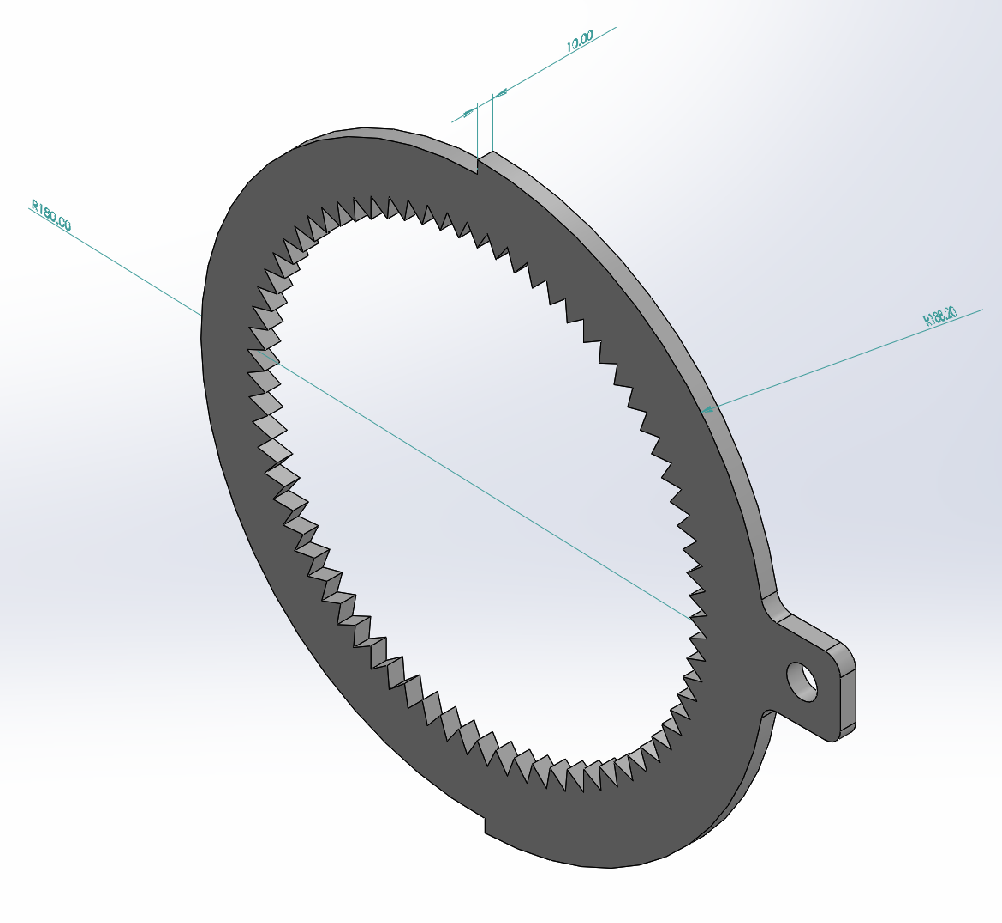
\includegraphics[height=0.25\textwidth]{gearCAD}
				\caption{Aluminium gear used as the outside of the planetary gear, with dimensions}
				\label{gearCAD}
				\columnbreak
				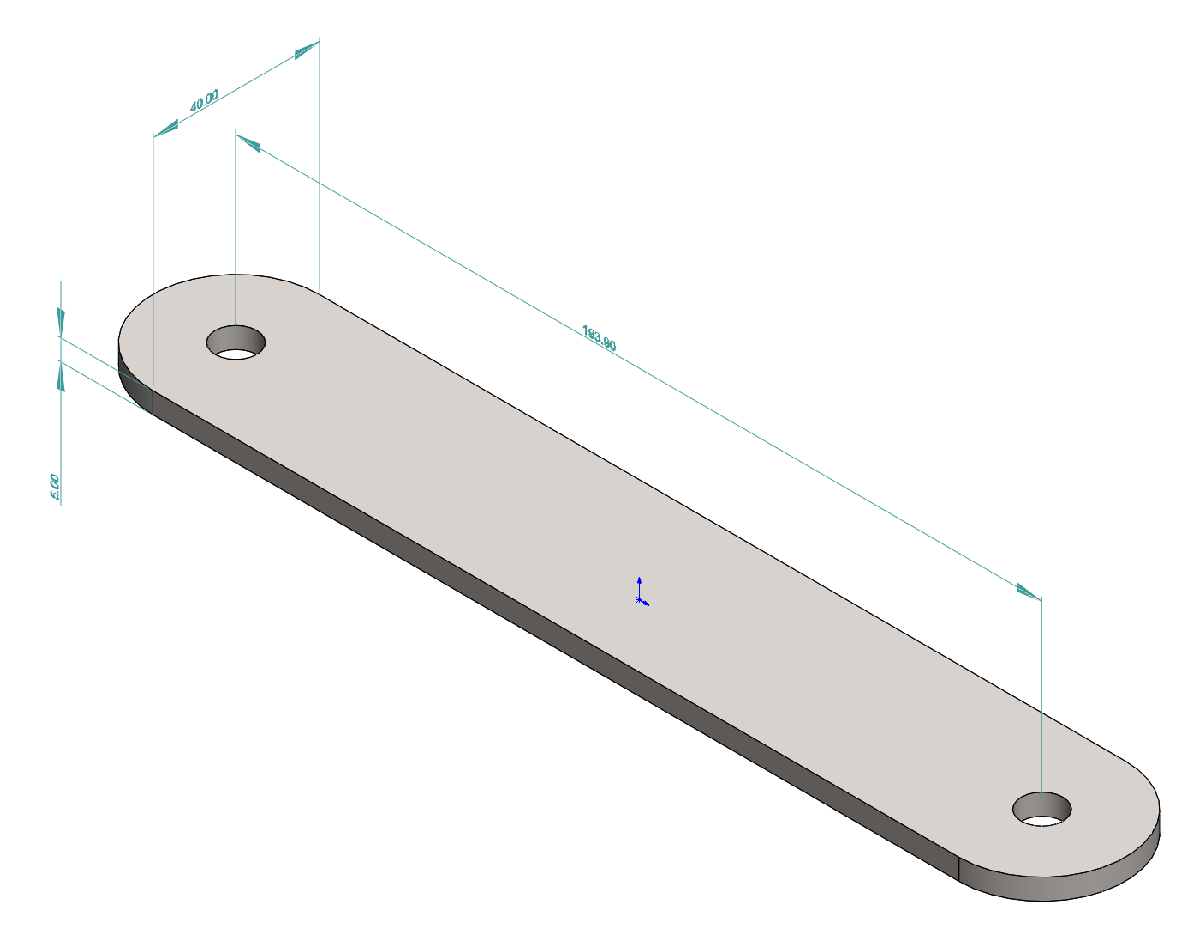
\includegraphics[height=0.25\textwidth]{shortLinkCAD}
				\caption{Stainless steel short link of the leg mechanism with dimensions}
				\label{shortLinkCAD}
				\columnbreak
				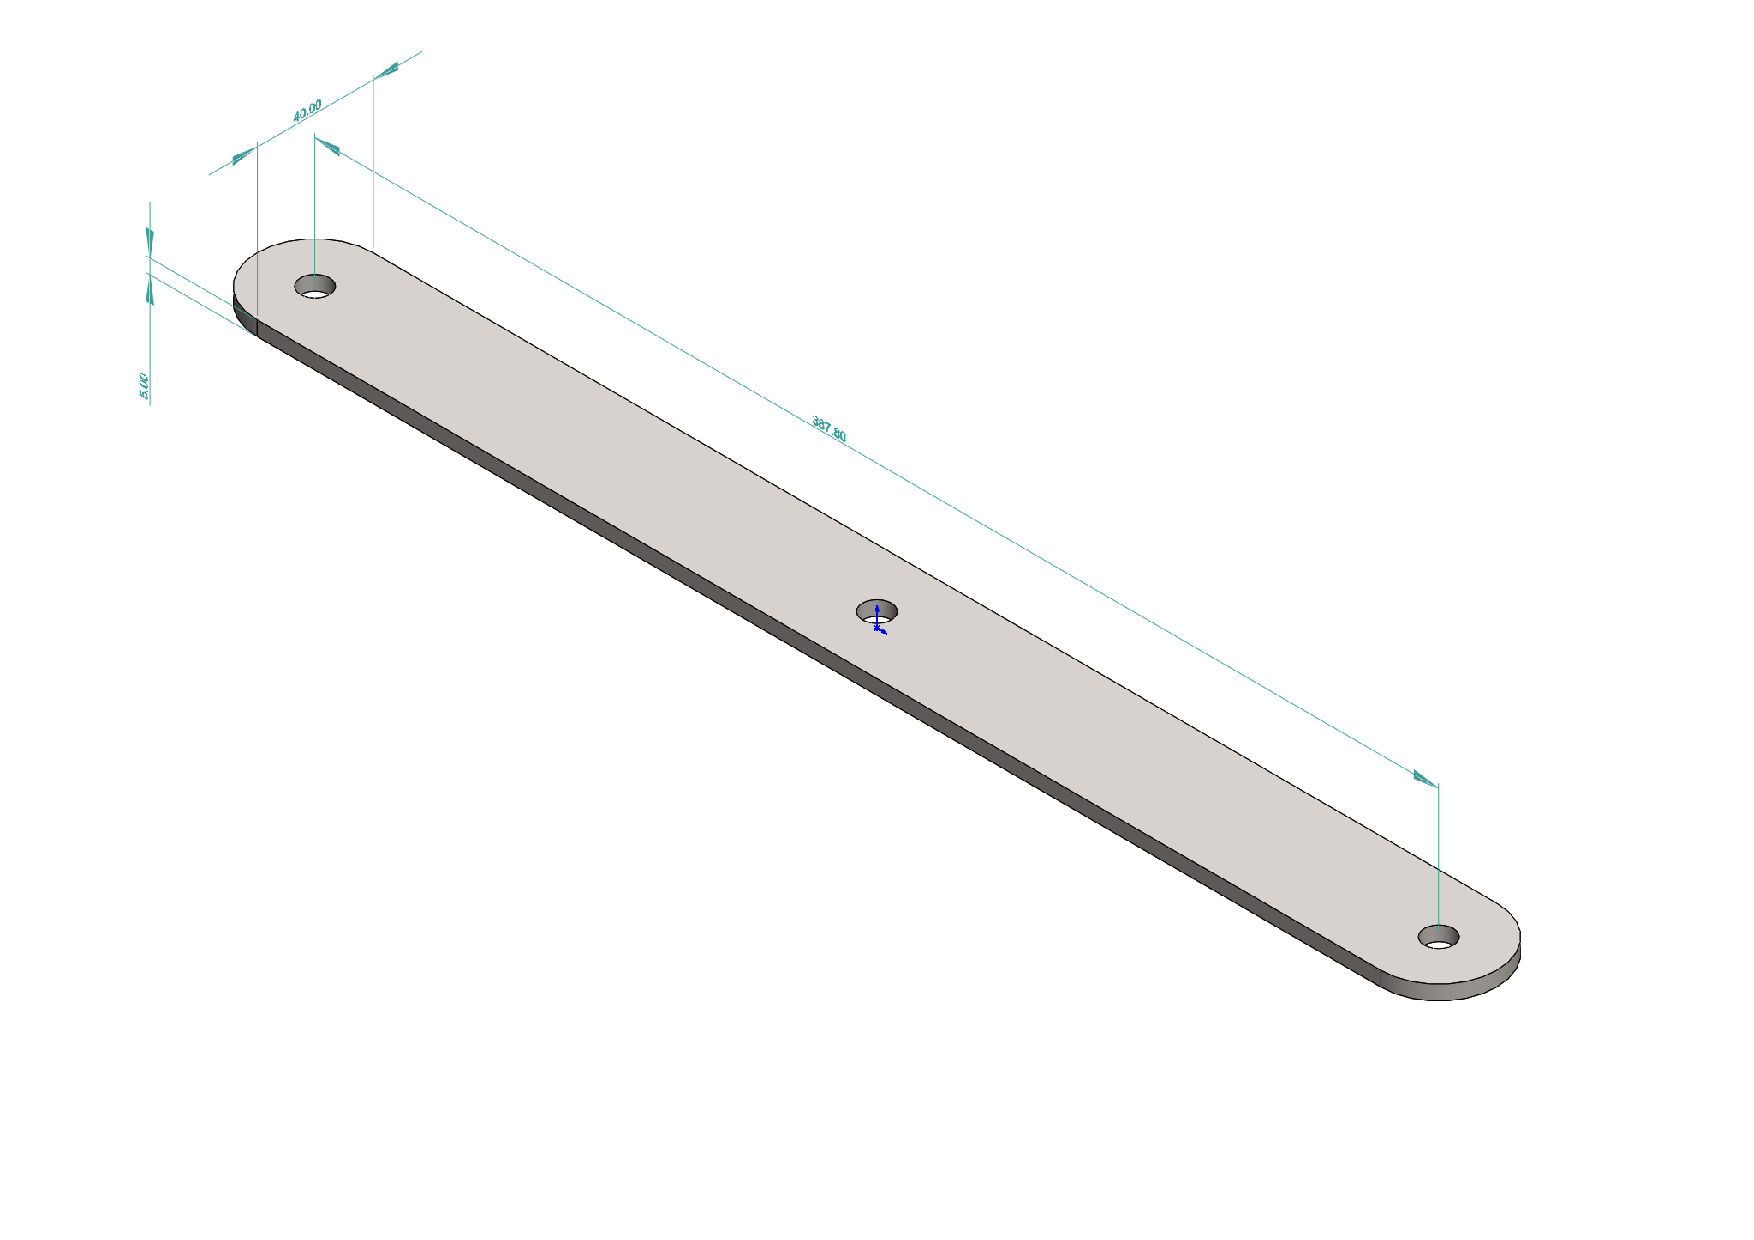
\includegraphics[height=0.25\textwidth]{longLinkCAD}
				\caption{Stainless steel long link of the leg mechanism with dimensions}
				\label{longLinkCAD}
			\end{multicols}
		\end{figure}
		The remaining components of the locomotion system were estimated using the 3D CAD models, shown in \hyperref[gearCAD]{Figures \ref*{gearCAD}, \ref*{shortLinkCAD} \& \ref*{longLinkCAD}} to estimate their volume.
		The leg pieces were assumed to be made out of stainless steel, and the gear was to be made of aluminium.
		The density of stainless steel is $7900$ kg m\textsuperscript{-3}\textsuperscript{\cite{HLT}}, so the longer link weighs $0.653$ kg and the shorter link weighs $0.350$ kg.
		Thus, a single leg, which is made up of 2 short links and 2 longer links, weighs $2.00$ kg, bringing the total contribution of the three legs to $6.02$ kg for the whole robot.
		The density of aluminium was assumed to be $2700$ kg m\textsuperscript{-3}\textsuperscript{\cite{HLT}}, which makes the weight of a single gear $3.42$ kg, and there are 4 inside the robot, bring the total weight up to $13.68$ kg
		This could be mitigated by refining the design, as this is a very rough sketch of the gear, and is probably thicker than would be necessary in reality.
		
		\subsection{Power}
		
		\subsection{Sensing}
		
		\subsection{Communications}
		
		\subsection{External Hardware}
		% Does not need to be included in the weight calc obviously
			
	\section{Industry Analysis}
		
		It was decided to use the Porter's Five Forces model\textsuperscript{\cite{porter2008five}} to analyse the in-pipe inspection robot industry, in order to provide a systematic analysis of the existing and possible threats to our company in the future.
		
		\subsection[Threat of Entry]{Threat of New Entry}
				
		\subsection[Power of Suppliers]{Power of Suppliers}
		
		\subsection[Power of Buyers]{Power of Buyers}
		
		\subsection[Threat of Substitutes]{Threat of Substitutes - Jim Laney}
			
			The threat of substitutes in the in-pipe inspection robot industry is medium, as there are many established substitutes which currently dominate pipe inspection services.
			\\
			The main threat is the manual inspection of pipelines as these can inspect all kinds of pipes, just like robotic solutions and have a much lower up front cost.
			As well as this, manual inspection has the advantage of familiarity as it is an established practice which gas pipe companies know they can rely on.
			Manual inspection uses different methods for inspecting pipes dependent on the the kind of damage being inspected for.
			\\
			For external corrosion inspection, a pre-assessment is performed, followed by both indirect and direct inspection techniques being used, the latter of which requires excavation to occur for that section of the pipe\textsuperscript{\cite{kishawy2010review}}. 
			For internal corrosion inspection, a similar process is followed, with pipes that have the greatest inclination being inspected first to identify the location of localised corrosion. 
			However, both these methods require excavation in order to confirm the location of the corrosion, which is disruptive, especially in urban environments.
			\\
			When checking for cracks manual inspection can typically only find these when a leak has occurred, as there is otherwise very little change in behaviour of the gas inside the pipe.
			Thus, manual methods rely on constant assessment of conditions within the pipe, such as the mass-balance method, pressure-drop method and using gas smelling dogs\textsuperscript{\cite{kishawy2010review}}.
			Ground penetrating radar is also used as another method for looking for cracks without excavation, but visual inspection is also typically used to ensure accuracy of the readings, which does require excavation.
			Computer models can also be used to predict the behaviour of the pipeline in order to predict faults, but as this requires modelling of complex fluid dynamics, these are not always reliable.
			\\
			Pipeline Inspection Gauges (PIGs) are the other main substitute to robotic in-pipe inspection, as these are passive devices which are forced along the pipeline by the gas flow.
			However, PIGs are uncontrollable and cannot operate in pipelines containing sharp bends\textsuperscript{\cite{mills2017advances}}, making them unsuitable for urban pipelines.
			As such the threat from PIGs is minimal since we have specifically chosen to enter an area where they are not currently suitable, although it is possible that more advanced PIGs may be developed in the future which compete in the area of urban pipelines.
		
		\subsection[Rivalry Among Existing Competitors]{Rivalry Among Existing Competitors}
		
	\section{Customer Industry Analysis}
		% Insert Monty's P5F here
		Since we have only one customer industry, we felt it was important to analyse the safety and sustainability of that industry to ensure that our business was secure.
		We once again used the Porter's Five Forces model\textsuperscript{\cite{porter2008five}} to analyse the gas pipeline inspection industry.
			
		\subsection[Threat of Entry]{Threat of New Entry}
				
		\subsection[Power of Suppliers]{Power of Suppliers}
		
		\subsection[Power of Buyers]{Power of Buyers}
		
		\subsection[Threat of Substitutes]{Threat of Substitutes}
			
			
		
		\subsection[Rivalry Among Existing Competitors]{Rivalry Among Existing Competitors}
	
	\pagebreak		% Temp page break for references - might end up replacing with a multicolumn environment later
	
	% In order to make a reference to an entry in the bibliography, use \cite{}
	% TexStudio will suggest names from the bib file - not sure about overleaf but otherwise use the first entry in the string
	% Make sure bibliography is set to use BibTex rather than BibLatex
	% See mybib.bib for an example bib file format - most things should be able to give it to you in this format
	% Our actual bibliography will be 3YPbib.bib
	% Currently using google scholar default ids - should help prevent duplication of references but will need to be checked
	
	% For websites use the misc tag - see how I've done rsproLinear - the author is in 2 brackets so it doesn't get made into initials
	
	%\nocite{*} 				% By default Latex will not show uncited references, uncomment this line to show all references in the bib file
	
	\begingroup\onehalfspacing
		{\small
			\bibliographystyle{ieeetr}
			\bibliography{3YPbib}
		}
	\endgroup

\end{document}
